\documentclass[a4paper, 12pt, oneside]{report}

\usepackage[utf8]{inputenc}
\usepackage{lmodern}
\usepackage{layout}
\usepackage{emptypage}
\usepackage{fancyhdr}
\usepackage{fancyref}
\usepackage{fancyvrb}
\usepackage{subcaption} % subfiguras
\usepackage{caption}
\usepackage{mathtools}
\usepackage{hyperref}
\usepackage[a4paper,top=3cm, bottom=3cm, inner=2.5cm, outer=2.5cm]{geometry}
\usepackage{listings}
\usepackage[english]{babel}
\usepackage{url}
\usepackage{color}
\usepackage[backend=bibtex,style=ieee,natbib=true]{biblatex}
\addbibresource{Bibliography.bib}
\usepackage{amsmath}
\usepackage{algorithm}
\usepackage{amsmath}
\usepackage[noend]{algpseudocode}

\definecolor{codegreen}{rgb}{0,0.6,0}
\definecolor{codegray}{rgb}{0.5,0.5,0.5}
\definecolor{codepurple}{rgb}{0.58,0,0.82}
\definecolor{backcolour}{rgb}{0.95,0.95,0.92}

\lstset{frame=single,
	language=Python,
	aboveskip=3mm,
	belowskip=3mm,
	showstringspaces=false,
	columns=flexible,
	basicstyle={\small\ttfamily},
	numbers=none,
	backgroundcolor=\color{backcolour},   
	commentstyle=\color{codegreen},
	keywordstyle=\color{blue},
	numberstyle=\color{codepurple},
	stringstyle=\color{magenta},
	breaklines=true,
	breakatwhitespace=true,
	tabsize=3
}

\usepackage[acronym,nomain]{glossaries}
\newacronym{ai}{AI}{artificial intelligence}
\newacronym{ann}{ANN}{artificial neural network}
\newacronym{ml}{ML}{machine learning}
\newacronym{cnn}{CNN}{convolutional neural network}
\newacronym{hdf5}{HDF5}{Hierarchichal Data Format version 5}
\newacronym{gui}{GUI}{graphical user interface}
\newacronym{mnist}{MNIST}{Modified National Institute of Standards and Technology}
\newacronym{lmdb}{LMDB}{Lightning Memory-Mapped Database}
\newacronym{relu}{ReLU}{rectified linear unit}
\newacronym{roi}{ROI}{region of interest}
\makeglossaries

%\usepackage{titlesec}
\makeatletter
\renewcommand{\@makeschapterhead}[1]{
  \vspace*{0\p@}%
  {\parindent \z@ \raggedright
    \normalfont
    \interlinepenalty\@M
    \Huge \bfseries  #1\par \nobreak
    \vskip 15\p@
  }}
\makeatother

\renewcommand{\baselinestretch}{1.4}
\setlength{\headheight}{16pt} 

\pretolerance=1000

\chead[]{}
\rhead[]{}
\renewcommand{\headrulewidth}{0.5pt}

\pagestyle{empty}

\title{Vehicle Detection using Deep Learning}
\author{David Pascual Hernández}

\begin{document}
%%%%%%%%%%%%%%% Cover %%%%%%%%%%%%%%%%%%%%
\begin{titlepage}
	
	\begin{center}
		
		\begin{figure}[htb]
			\begin{center}
				
\includegraphics[width=0.6\linewidth]{figures/logo}
			\end{center}
		\end{figure}
		
		\vspace{10mm}
		
		\begin{Large}
			\textbf{ESCUELA TECNICA SUPERIOR DE INGENIERÍA DE TELECOMUNICACIÓN}
			\vspace{10mm}
		\end{Large}
		
		\begin{Large}
			Grado en Ingeniería en\\ \vspace{2mm} Sistemas Audiovisuales y Multimedia
		\end{Large}
		
		\vspace{10mm}
		
		\begin{large}
			\textbf{Trabajo Fin de Grado}
		\end{large}
		\vspace{25mm}
		
		\begin{huge}
			Study of Convolutional Neural Networks with Keras
		\end{huge}
		
		\vspace{25mm}
		
		\begin{large}
			\textbf{Autor}: David Pascual Hernández
			
			\textbf{Tutor}: José María Cañas Plaza
			
			\textbf{Co-tutor}: Inmaculada Mora Jiménez 
			
			\vspace{10mm}
			
			Curso académico 2016/2017
		\end{large}
		
		\vspace{10mm}
		
	\end{center}
	
\end{titlepage}

\pagebreak
\thispagestyle{empty}
\vspace*{12cm}

\begin{flushright}
	
	
\includegraphics[height=1.0cm]{figures/CC-BY-SA.png}
	
	\vspace*{0.5cm}
	
	\copyright 2017 David Pascual Hernández
	
	\vspace*{0.3cm}
	
	Esta obra está distribuida bajo la licencia de 
	
	``Reconocimiento-CompartirIgual 4.0 Internacional (CC BY-SA 4.0)''
	
	de Creative Commons.
	
	\vspace{0.2cm}
	
	Para ver una copia de esta licencia, visite
	
	http://creativecommons.org/licenses/by-sa/4.0/ o envíe
	
	una carta a Creative Commons, 171 Second Street, Suite 300,
	
	San Francisco, California 94105, USA.
	
\end{flushright}

\pagenumbering{Roman}

%%%%%%%%%%%%%%% Acknowledgements %%%%%%%%%%%%
%\chapter*{}
%\pagenumbering{Roman} % para comenzar la numeracion de paginas en numeros romanos
%\begin{flushright}
%	\textit{``I'm afraid that the following syllogism may be used by some in the future:\\	Turing believes machines think.\\	Turing lies with men.\\	Therefore machines do not think."\\  —Alan Turing, 1952}
%\end{flushright}

\chapter*{Agradecimientos}
Este trabajo de fin grado supone para mí la culminación de una dura etapa de aprendizaje de la que, sin duda alguna, he salido reforzado. Reforzado no sólo por los conocimientos adquiridos, si no por las herramientas brindadas para adquirir aquellos que están por llegar. Hasta hace poco desconocía la existencia de materias que a día de hoy me apasionan profundamente. Me siento privilegiado por tener la oportunidad de ser espectador de los cambios que estas materias están produciendo en el mundo, y me emociona trabajar para intentar ser partícipe de ellos. Estos descubrimientos son resultado directo del buen hacer de muchos de los docentes que he conocido estos últimos años. En especial, me gustaría dar las gracias a Inmaculada y Jose María. Su guía incondicional en el desarrollo de este trabajo, lo ha convertido en una experiencia fructífera y gratificante. También quiero dar las gracias a Nuria, compañera de fatigas en estos últimos meses. Gracias a vosotros puedo presumir de estar aprendiendo con los mejores.

Esta aventura ha estado llena de retos y obstáculos, y no tengo ningún reparo en reconocer que jamás habría sido capaz de superar muchos de ellos sin ayuda. En este sentido, quiero dar las gracias a todos los compañeros en los que me he apoyado para superarlos. En particular, agradezco enormemente a Marco y Abel haber compartido conmigo su amistad. Larga vida al \emph{metal}. 

Más alla de lo académico, tengo la fortuna de haber disfrutado de la mejor compañía que pueda imaginar. Por su excelente conversación, su ingenio, su paciencia y su sapiencia, me faltan horas en el día para dar las gracias a Andrés y Alejandra. Os quiero.

Los últimos años, han sido una convulsión de viajes, proyectos, satisfacciones y decepciones. Es difícil digerir estos cambios cuando no encuentras la forma de comunicarte y de hacer comprender a los demás aquello que te aflige. Por suerte, entre esa maraña de cambios, me crucé con Carolina. Gracias por tu bondad y tu forma de ver el mundo. Te quiero.

Por último, doy las gracias a mi familia, y especialmente a mis padres, Virginia y David. Todo lo que he aprendido en la vida puedo dividirlo en dos grandes grupos: aquello que me habéis enseñado vosotros y aquello que me habéis enseñado a aprender.

%%%%%%%%%%%%%%% Resumen %%%%%%%%%%%%%%%%%%%%
\chapter*{Resumen}
El \emph{reconocimiento de objetos} en imágenes ha sido un problema recurrente en la historia de la \emph{visión artificial}. Gracias a la inclusión de algoritmos basados en aprendizaje máquina y, más recientemente, de las técnicas de \emph{aprendizaje profundo}, se han enfrentado con éxito problemas como el reconocimiento de señales de tráfico o la videovigilancia. En concreto, las \emph{redes neuronales convolucionales} se han convertido en la punta de lanza de este tipo de algoritmos en los últimos años. Su eficacia en la resolución de problemas como los anteriormente mencionados resulta indiscutible en muchos casos, lo que poco a poco está favoreciendo su uso en aplicaciones comerciales. A pesar de ello, siguen siendo acusadas de actuar como una caja negra o \emph{black box}, ya que por lo general su aprendizaje es un proceso opaco y difícil de interpretar.

Por todo ello, este trabajo de fin grado tiene como metas el \emph{estudio detallado} de las redes neuronales convolucionales y su \emph{aplicación} en el abordaje de un determinado problema. En este sentido, se desarrollará un \emph{clasificador de dígitos manuscritos en tiempo real}. Para entrenar e implementar las redes neuronales convolucionales, se empleará la plataforma \emph{Keras}. El proyecto comienza con el análisis de una red neuronal convolucional de ejemplo proporcionada por dicha plataforma. Posteriormente, se procede al desarrollo del \emph{componente} clasificador de dígitos. Este componente adquiere imágenes desde una fuente de vídeo, las clasifica gracias a una red neuronal de Keras y muestra el resultado en una interfaz gráfica. Además, se ha conformado un \emph{banco de pruebas} en el que se incluyen bases de datos para alimentar las redes neuronales convolucionales y herramientas para calcular y visualizar parámetros de evaluación. Por último, gracias a las herramientas del banco de pruebas, se discutirán los \emph{efectos que produce el aprendizaje sobre el desempeño} de distintas redes neuronales, y aquella que mejores resultados arroje será integrada en el componente clasificador de dígitos para lograr una mayor robustez.

Los resultados obtenidos ponen de manifiesto el gran potencial de las redes neuronales convoluciones y proyectan algo de luz sobre su aprendizaje, dejando abierta la puerta a su empleo en la resolución de problemas más complejos.

%%%%%%%%%%%%%%% Summary %%%%%%%%%%%%%%%%%%%%
\chapter*{Summary}
\emph{Object recognition} has been a recurring problem in the history of \emph{computer vision}. Thanks to the inclusion of machine learning and, recently, \emph{deep learning} algorithms, issues like traffic sign recognition and video surveillance have been successfully addressed. In particular, \emph{convolutional neural networks} have become the spearhead of this kind of algorithms in the last few years. In many cases, their effectiveness solving issues like the ones mentioned before can't be denied, which has enabled their usage in commercial applications. Nevertheless, convolutional neural networks keep being accused of acting like \emph{black boxes}, because their learning process is usually very opaque and hard to interpret.

For all of these reasons, this final degree project aims to serve as a \emph{detailed study} of convolutional neural networks and their \emph{implementation} for solving a certain problem. In this case, a \emph{real-time handwritten digits classifier} will be developed. These objectives will be faced employing the \emph{Keras} platform. The project starts with the analysis of a convolutional neural network example provided by the aforementioned library. Then, the digit classifier \emph{component} is discussed. This component acquires images from a video source, classifies them thanks to a neural network built with Keras and displays the result in a graphical user interface.  Besides that, a \emph{test bench} has been developed. It is formed by datasets that will feed the convolutional neural networks and tools for computing and visualizing evaluation parameters. Finally, thanks to the tools created for the test bench, the effects of the learning process in the performance of different neural networks will be discussed, and the one that achieves better results will be integrated within the digit classifier component to accomplish a greater robustness.

The results obtained reveal the great potential of the convolutional neural networks and cast some light on how they are able to learn what they learn, opening the door for their usage in the settlement of more complex problems.

%%%%%%%%%%%%%%% Índices %%%%%%%%%%%%%%%%%%%%
\tableofcontents
\listoffigures % Í­ndice de figura
\listoftables
\printglossaries
\cleardoublepage

%%%%%%%%%%%%%%% Chapters %%%%%%%%%%%%%%%%%%
\pagestyle{fancy}
\pagenumbering{arabic}
\setlength{\parindent}{6mm}

\lhead[]{CHAPTER \thechapter. ABSTRACT}
\chapter{Introduction}\label{ch:introduction}
\section{Context and motivation}
Since the term \textbf{\gls{ai}} was coined at the Dartmouth Conference in 1956~\cite{mccarthy2006proposal} until nowadays, this field of computer science has developed at a great pace. During this time, its contributions to robotics and computer vision have brought machines that can solve certain tasks as well as humans and, in some, cases even surpass human performance. In order to understand the context in which this project has been developed, the fields and subfields that have lead to the birth of \textbf{\glspl{cnn}} are going to be defined, trying to clarify the differences between them and how they are related to each other. 
\begin{description}
	\item[\textbf{Artificial intelligence}] "It is the subfield of computer science devoted to developing programs that enable computers to display behavior that can (broadly) be characterized as \textbf{intelligent}"~\cite{sep-logic-ai}, where \textit{intelligent} refers to the ability of perceiving the environment and acting consequently, trying to maximize the chances of achieving a certain goal~\cite{Russell:2003:AIM:773294}.
\end{description}
\begin{description}
	\item[\textbf{Machine learning}] According to a quote attributed to Arthur Samuel, it is the "field of study that gives computers the \textbf{ability to learn} without being \textbf{explicitly programmed}". Given this definition, it can be asserted that \gls{ml} is a subfield of \gls{ai}, because computers that have the ability to learn will exhibit an \textit{intelligent} behaviour, but displaying an \textit{intelligent} behaviour doesn't necessarily mean to learn. For instance, \textbf{Deep Blue} chess-playing system can be considered \textit{intelligent} as it achieves a \textbf{human comparable performance}, but instead of actually learning to play, it was hard-coded with a function that evaluated the board positions~\cite{Goodfellow-et-al-2016}.  
\end{description}
\begin{description}
	\item[Artificial neural networks] They are a computational approach that tries to model the way a \textbf{biological neural network} solves problems. As it can be seen in Figure~\ref{fig:ANN}, they're formed by layers of interconnected \textbf{neural units}.
	\begin{figure}
		\centering
		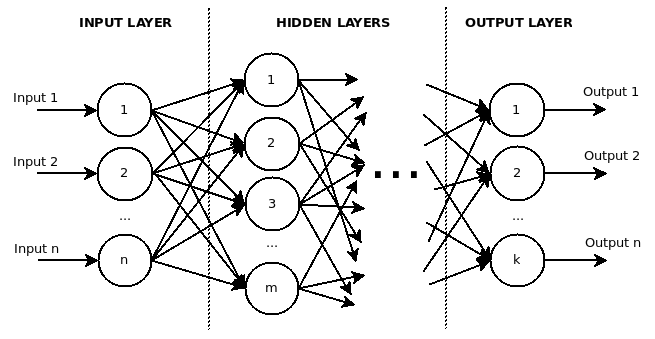
\includegraphics[width=0.8\linewidth, keepaspectratio]{figures/ANN.png}
		\caption{Basic architecture of an artificial neural network.}
		\label{fig:ANN}
	\end{figure}
	
	In \glspl{ann}, each neural unit sums the weighted input signals and apply an \textbf{activation function} that can be linear or non-linear (see Figure~\ref{fig:unit}). The result of this operation is transferred to the neurons of the next layer. During training, weights are updated based on a \textbf{learning rule} that will try to minimize the difference between the current output and the desired one. As \glspl{ann} are able to learn from experience, they're classified within the \gls{ml} field.
	\begin{figure}
		\centering
		\includegraphics[width=0.8\linewidth, keepaspectratio]{figures/unit.png}
		\caption[A neural unit.]{A neural unit (image extracted from~\cite{neural-unit}).}
		\label{fig:unit}
	\end{figure}
\end{description}
\begin{description}
	\item[\textbf{Deep learning}] It is a branch of \gls{ml} which is based on algorithms that share the following properties~\cite{deep-learning-methods-and-applications}:
	\begin{itemize}
		\item \textbf{Multiple layers} of \textbf{non-linear} processing units.
		\item The supervised or unsupervised \textbf{hierarchical learning} of feature representations in each layer.
	\end{itemize}
	
	Although the term \textit{deep learning} is not explicitly linked to \glspl{ann}, in practice, we could talk about deep learning as a subset of neural networks algorithms that share the properties mentioned above. 
\end{description}
\begin{description}
	\item[\textbf{Convolutional neural networks}] They are "neural networks that use \textbf{convolution} in place of general matrix multiplication in at least one of their layers"~\cite{Goodfellow-et-al-2016}. \glspl{cnn} are specifically designed to process data that has a \textbf{grid-like topology}, like images and audio. In a few years, they have become one of the most promising subfields of \gls{ml}, outperforming the results achieved by the previous algorithms in the most popular benchmarks for tasks like object classification, object detection and natural language processing. The details about how \glspl{cnn} work will be the deeply discussed in the following chapters.
\end{description}

\begin{description}
	\item[\textbf{Computer vision}] It is a field of computer science which "aims to build \textbf{autonomous systems} which could perform some of the tasks that the \textbf{human visual system} can perform"~\cite{huang1996computer}. In order to build autonomous systems, computer vision applications have to deal with image acquisition, processing and analysis. Computer vision has always been closely related to \gls{ai} and \gls{ml}, and in the last years, the integration of deep learning algorithms (e.g. \glspl{cnn}) in computer vision applications has lead to major advances in the field.
\end{description}

There are multiple \textbf{motivations} behind this project. On one hand, I am very passionate about \textbf{computer vision}, because of its great implications in everyday life. For instance, it is involved in medical imaging, surveillance, augmented reality, automatic inspection in manufacturing, self-driving cars... and the list goes on and on. On the other hand, all of the applications that have just been mentioned, have benefited from the inclusion of \textbf{deep learning} in computer vision. It is really exciting to see how many researchers are currently working in the field. Of course, this is not a coincidence. The great results achieved with these new algorithms has boosted the growth of \gls{ai} in the last years and has normalized its usage in \textbf{commercial applications}. However, everything has its ups and downs. There is a lot of people worried about the so-called \textbf{\textit{black box} problem} in deep learning~\cite{black-box}, i.e., how machines are actually learning to do what they do. In this work, besides developing a real-world application to show how powerful \glspl{cnn} are, we're going to try to cast some light into the aforementioned \textit{black box}. 

\section{Objectives}\label{sec:objectives}
The ultimate objective of this project is to fully understand \glspl{cnn} in order to integrate them in a computer vision application that must be able to solve a real-world task, specifically a \textbf{real-time handwritten digits classifier}. This main objective has been divided in the following sub-objectives: 
\begin{itemize}
	\item Accomplishing a \textbf{deep understanding} of how a basic \gls{cnn} work, analyzing its main layers, the learning process and the particularities of building this kind of networks with \textbf{Keras library}.
	\item Developing a \textbf{benchmark} which allows the comparison of the performance achieved by the \glspl{cnn}. This benchmark must provide the input data and the tools required to visualize and evaluate the results.
	\item Finding the \textbf{optimal \gls{cnn}} evaluating the results achieved employing new data, new architectures and different learning processes.
	\item Building a \textbf{component}, aided by JdeRobot middleware, which must integrate the \gls{cnn} to classify the handwritten digits images.
\end{itemize}

\section{Methodology}
The development of this project has been followed weekly by the tutors. In the \textbf{weekly meetings}, the work done in the previous week was discussed and new milestones were set for the following one. This methodology has allowed a continuous feedback, which has lead to a better understanding of the topic. Besides that, thanks to the weekly meetings the workload has been constant during these months. 

Additionally, the following tools have been employed to keep track of the project progress:
\begin{itemize}
	\item \textbf{GitHub}. All the code written in this project is available in GitHub and has been  frequently updated. In the following link, the main repository can be accessed:
	\url{https://github.com/RoboticsURJC-students/2016-tfg-david-pascual}
	\item \textbf{JdeRobot MediaWiki}. It has been used as a logbook of the progress of this project. It can be accessed in the following link:
	\url{http://jderobot.org/Dpascual-tfg}
\end{itemize}

In Figure~\ref{fig:gantt}, a \textbf{Gantt chart} with the number of weeks dedicated to every task in the project can be seen.
\begin{figure}
	\centering
	\includegraphics[width=0.9\linewidth, keepaspectratio]{figures/gantt.png}
	\caption{Gantt chart.}
	\label{fig:gantt}
\end{figure}

\section{Project structure}
For ease of reading, the structure followed in the writing of this project and how the chapters are related to each other are going to be explained in this section.

\begin{description}
	\item[Introduction] This chapter starts with a brief introduction to the main fields in which \glspl{cnn} are based and the motivations behind the project. Then, the objectives, the methodology followed to meet these objectives and the structure of the project are presented.
	\item[Framework] The software that was already there before the project is described here. It's specially significant the section about Keras library, its main functionalities and the theory behind its core layers and learning process.
	\item[Digit classifier] In this chapter, an example of a \gls{cnn} built with Keras for handwritten digits classification is analyzed and then, the working of the component, in which the \gls{cnn} is integrated, is explained.
	\item[Benchmark] The datasets that will be used for training new models and the tools that will be employed to evaluate and visualize the results are described in this chapter.
	\item[Evaluation] Taking as a starting point the \gls{cnn} that was analyzed in the \textit{Digit classifier} chapter, new models will be created. The performance of these new models will be evaluated with the tools developed in the \textit{Benchmark} chapter.
	\item[Conclusions] Finally, all the valuable conclusions reached during the development of the project will be summarized and possible further works will be proposed.
\end{description}
\lhead[]{CHAPTER \thechapter. FRAMEWORK}
\chapter{Framework}\label{ch:framework}
This chapter serves as a way to introduce the tools that have been employed during the development of this project. All of them are \textbf{open-source}. The transparency provided by the open-source platforms is a major advantage, because the software can be joined together and adapted to our specific applications, which are mainly written in \textbf{Python} \footnote{\url{https://www.python.org/}}.

\section{Keras}\label{sec:keras}
As stated by \textbf{Keras} documentation~\cite{chollet2015keras}: "Keras is a high-level \textbf{neural network library}, written in Python and capable of running on top of either TensorFlow or Theano". TensorFlow and Theano are open-source libraries for numerical computation optimized for GPU and CPU that Keras treats as its \textit{backends}. In this project, Keras is running on top of \textbf{Theano} \footnote{\url{http://deeplearning.net/software/theano/index.html}} optimized for CPU, but it's quite easy to switch from one backend to another.

In the following sections, the main elements that make up a neural network built with Keras are going to be analyzed, starting with the \textbf{\textit{model} object}, its core component.

\subsection{Models}\label{subsec:models}
Every neural network in Keras is defined as a \textbf{\textit{model}}. For those models which can be built as a stack of \textit{layers} (see Section~\ref{subsec:layers}), Keras provides the \textbf{\textit{.Sequential()} object}. An example of a sequential model built with Keras can be seen in the following chapter in Figure~\ref{fig:model}. It is also possible to build more complex models with multiple outputs and shared layers using the \textbf{Keras functional API}.

Sequential models have several methods, and the following ones are essential for the learning process:
\begin{description}
	\item[\textit{.compile()}] It configures the \textbf{learning process}. It's main arguments are:
	\begin{itemize}
		\item \textbf{\textit{loss}}: name of the \textbf{cost function} employed to check the difference between the predicted labels and the real ones. In this project, the \textbf{categorical cross-entropy}, also known as log loss, has been used. This function returns the cross-entropy between an approximating distribution $q$ and a true distribution $p$~\cite{theano} and it's defined as:
		\begin{equation}\label{eq:categorical_crossentropy}
		H(p,q)=-\Sigma_{x}p(x)\log(q(x))
		\end{equation}		
		Other loss functions such as mean squared error (MSE), mean absolute error and hinge are also provided by Keras.
		
		\item \textbf{\textit{optimizer}}: name of the optimizer that will update the weights values during training in order to minimize the loss function. The chosen algorithm for this task is \textbf{ADADELTA}. This optimizer is an extension of the \textbf{gradient descent} optimization method that has the particularity of adapting the learning rate during training with no need of manual tuning. According to the paper in which it is defined~\cite{DBLP:journals/corr/abs-1212-5701}, it follows the next algorithm:		
		\begin{minipage}{\linewidth}
		\begin{algorithm}[H]
			\caption{Computing ADADELTA update at time $t$}\label{adadelta}
		  	\begin{algorithmic}[1]
		  		\Require{Decay rate $\rho$, Constant $\epsilon$}
		  		\Require{Initial parameter $x_1$}
		  		\State Initialize accumulation variables $E[g^2]_0=0, E[\Delta x^2]_0 = 0$
		  		\For{$t=1:T$} \Comment{Loop over \# of updates}
		  		\State Compute gradient: $g_t$
		  		\State Accumulate gradient: $E[g^2]_t=\rho E[g^2]_{t-1}+(1-\rho)g_t^2$
		  		\State Compute update: $\Delta x_t=-\frac{\mathrm{RMS}[\Delta x]_{t-1}}{\mathrm{RMS}[g]_t}g_t$
		  		\State Accumulate updates: $E[\Delta x^2]_t=\rho E[\Delta x^2]_{t-1}+(1-\rho)\Delta x_t^2$
		  		\State Apply update: $x_{t+1}=x_t+\Delta x_t$
				\EndFor
		  		\State \textbf{end for}
		  	\end{algorithmic}
		\end{algorithm}
		\end{minipage}\\
				
		Other optimization methods such as Adagrad, Adamax and Adam are also available.
		
		\item \textbf{\textit{metrics}}: name of the functions that must be evaluated during training and testing. The only one that is going to be computed with Keras through this project, besides the loss function, which is automatically computed, is \textbf{accuracy}. It is defined as the proportion of examples for which the model produces the correct output~\cite{Goodfellow-et-al-2016}.			
		Other measurements about the performance of the model are obtained with the \textbf{Scikit-learn} library (see Section~\ref{sec:sklearn}).
	\end{itemize}
\end{description}

\begin{description}
	\item[\textit{.fit()}] It trains the model. The following arguments are required:
	\begin{itemize}
		\item \textbf{\textit{x}, \textit{y}}: training samples and labels. They must be defined as \textbf{Numpy arrays}\footnote{\url{http://www.numpy.org/}}.
		
		\item \textbf{\textit{batch\_size}}: number of samples that are evaluated before updating the weights. It defaults to 32.
		
		\item \textbf{\textit{epochs}}: number of iterations over the whole dataset that are going to be executed. It defaults to 10.
		
		\item \textbf{\textit{callbacks}}: list of callbacks (see Section~\ref{subsec:callbacks}) that are going to be applied during training. It defaults to \textit{None}.
		
		\item \textbf{\textit{validation\_split} or \textit{validation\_data}}: in Keras, there are two alternatives to provide a validation dataset. On one hand, it is possible to pass the validation data as a Numpy array to the \textit{validation\_data} argument. On the other hand, a fraction of the training samples can be set as validation data through the \textit{validation\_split} argument. It's important to note that this new validation data won't be used for training anymore. \textit{validation\_data} and  \textit{validation\_split} arguments are mutually exclusive, so just one of them can be used.
		
		\item \textbf{\textit{shuffle}}: a boolean that determines whether to shuffle training data or not. 
	\end{itemize}
\end{description}

\begin{description}
	\item[\textit{.evaluate()}] It takes a set of samples and labels and evaluates the \textbf{model performance}, returning a list of the \textit{metrics} previously defined.
\end{description}

\begin{description}
	\item[\textit{.predict()}] It takes a sample and returns the label predicted by the model.
\end{description}

\begin{description}
	\item[\textit{.save()}] It stores the model into a \textbf{\gls{hdf5} file} (see Section~\ref{sec:hdf}), which will contain the weights, architecture and training configuration of the model.
\end{description}

\begin{description}
	\item[\textit{.load\_model()}] It loads a model from a \textbf{\gls{hdf5} file}.
\end{description}

\subsection{Layers}\label{subsec:layers}
As it has been said before, the models are usually built as a \textbf{stack of layers}. These layers are added to the model using the \textbf{\textit{.add()} method}, inside of which the kind of layer is declared and its particular parameters are set. Several kinds of layers are available, but only the ones that have been used in this project are going to be described.
\begin{description}
	\item[Convolutional layer] This particular layer is the one that turns the neural network into a \textbf{\gls{cnn}}. It is formed by a fixed number of \textbf{filters/kernels} with a fixed size. These filters are convolved along the input image, generating each one a \textbf{feature or activation map} which will tell us to what extent the feature learned by that particular filter is present in the input image~\cite{cs231n}. It's important to note that the depth of the filter will be equal to the number of channels of the input, which implies that each filter will generate just one activation map, instead of generating one for each channel. 
	
	Keras provides different kinds of convolutional layers depending on the input dimensions: \textit{Conv1D}, \textit{Conv2D} and \textit{Conv3D}. These are the main arguments required by Keras to define a convolutional layer:
	\begin{itemize}
		\item \textbf{\textit{filters}}: number of filters.
		
		\item \textbf{\textit{kernel\_size}}: width and height of the filters.
		
		\item \textbf{\textit{strides}}: how many pixels the filter must be shifted before applying the next convolution. It defaults to 1.
		
		\item \textbf{\textit{padding}}: it can be \textit{valid} or \textit{same}. If \textit{valid} mode is set, no padding is applied, resulting in a reduced output. However, if \textit{same} mode is set, the input will be padded with zeros in order to produce an output that preserves the input size. It defaults to \textit{valid}.
	\end{itemize}

	Figure~\ref{fig:convlayer} shows how the convolutional layers work. In Figure~\ref{fig:conv_a}, the filter $w_0$ (3x3x3) is convolved with the input image (5x5x3). As padding is set to 1 pixel around the input and the stride is equal to 2, the operation will return a 3x3 activation map. The same procedure is followed in Figure~\ref{fig:conv_b} with the filter $w_1$. It generates another 3x3 activation map, ending up with a 3x3x2 output. These images have been extracted from~\cite{cs231n}
	
	\begin{figure}
		\centering
		\begin{subfigure}{0.7\textwidth}
			\centering
			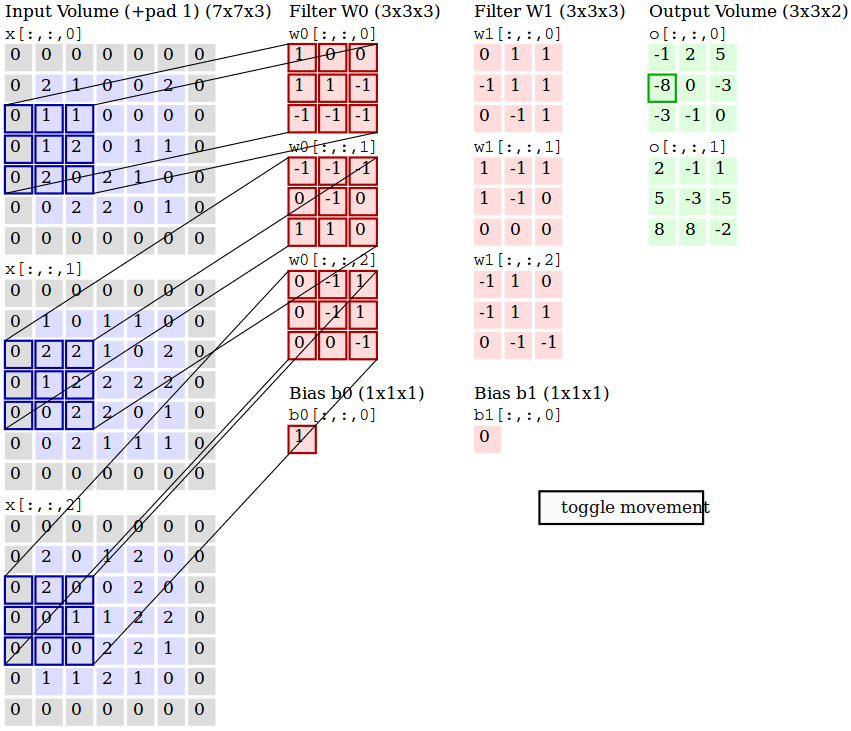
\includegraphics[width=1\linewidth]{figures/convlayer_anime1big.png}
			\caption{}\label{fig:conv_a}
		\end{subfigure}
		\begin{subfigure}{0.7\textwidth}
			\centering
			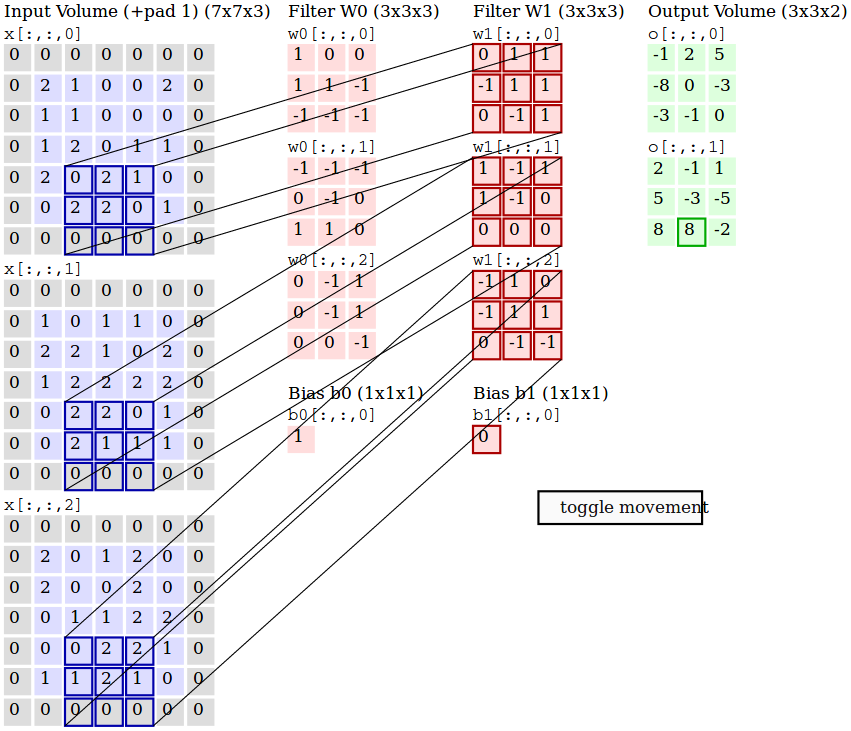
\includegraphics[width=1\linewidth]{figures/convlayer_anime2big.png}
			\caption{}\label{fig:conv_b}
		\end{subfigure}
		\caption{Convolutional layer.}
		\label{fig:convlayer}
	\end{figure}
	
\end{description}

\begin{description}
	\item[{Pooling layer}] It shifts a window of a certain size along the input image applying an operation (mean or maximum) that will return a \textbf{\textit{downsampled} version} of it, reducing the computational cost and avoiding overfitting~\cite{Scherer2010Evaluation}. Figure~\ref{fig:pooling} shows how the pooling operation is applied.

	\begin{figure}
		\centering
		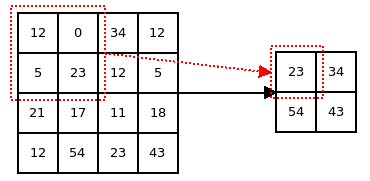
\includegraphics[width=10cm, keepaspectratio]{figures/pooling.png}
		\caption{Example of a max. pooling operation.}
		\label{fig:pooling}
	\end{figure}
	
	Depending on the dimensions of the input and the operation applied, Keras provides several pooling layers: \textit{MaxPooling1D}, \textit{MaxPooling2D}, \textit{MaxPooling3D}, \textit{AveragePooling1D}... The main arguments required by Keras to define these layers are:
	\begin{itemize}
		\item \textbf{\textit{pool\_size}}: size of the window that is shifted along the input. It can also be interpreted as the factor by which the input is going to be \textit{downsampled}.
		\item \textbf{\textit{strides}}: how many pixels the window must be shifted before applying the next operation.
	\end{itemize}
\end{description}

\begin{description}
	\item[Dense layer] Fully-connected layers in Keras are defined as \textit{Dense layers}. In a \textbf{fully-connected layer}, every neuron is connected to every activation (i.e. output) of the previous one~\cite{cs231n}. The main argument of this layer is:
	\begin{itemize}
		\item \textbf{\textit{units}}: number of neurons.
	\end{itemize} 
\end{description}

\begin{description}
	\item[Activation layers] In Keras models, an activation function can be declared as a layer itself or as an argument within the \textit{.add()} method of the previous layer. Keras provides several \textbf{activation functions}, such as sigmoid, linear, \gls{relu} and softmax. These are the ones that have been used during the development of this project:
	\begin{itemize}
		\item \textbf{\gls{relu}}: this activation function introduces \textbf{non-linearity} right after each convolutional layer, allowing the \gls{cnn} to learn more complex features. It's defined as:
		\begin{equation}\label{eq:relu}
		g(z)=\max(0,z)
		\end{equation}
		
		\item \textbf{Softmax}: this activation function is very useful when is placed after the \textbf{output layer} of classification tasks. It takes a vector of real values $z$ and returns a new vector of real values in the range [0,1]. The $N$ elements of the output vector can be considered \textbf{probabilities} because the softmax function ensures that they sum up to 1. It is defined as follows:
		\begin{equation}\label{eq:SoftMax}
		\mathrm{softmax}(z)_i=\frac{\exp(z_i)}{\Sigma_{j}{\exp(z_j)}} \quad \mathrm{for} \ j=1, ...,N
		\end{equation}
	\end{itemize}
	These equations and definitions have been extracted from~\cite{Goodfellow-et-al-2016}. Figure~\ref{fig:activations} shows these activation functions plotted in the interval $[-1,1]$.

	\begin{figure}
		\centering
		\begin{subfigure}{0.5\textwidth}
			\centering
			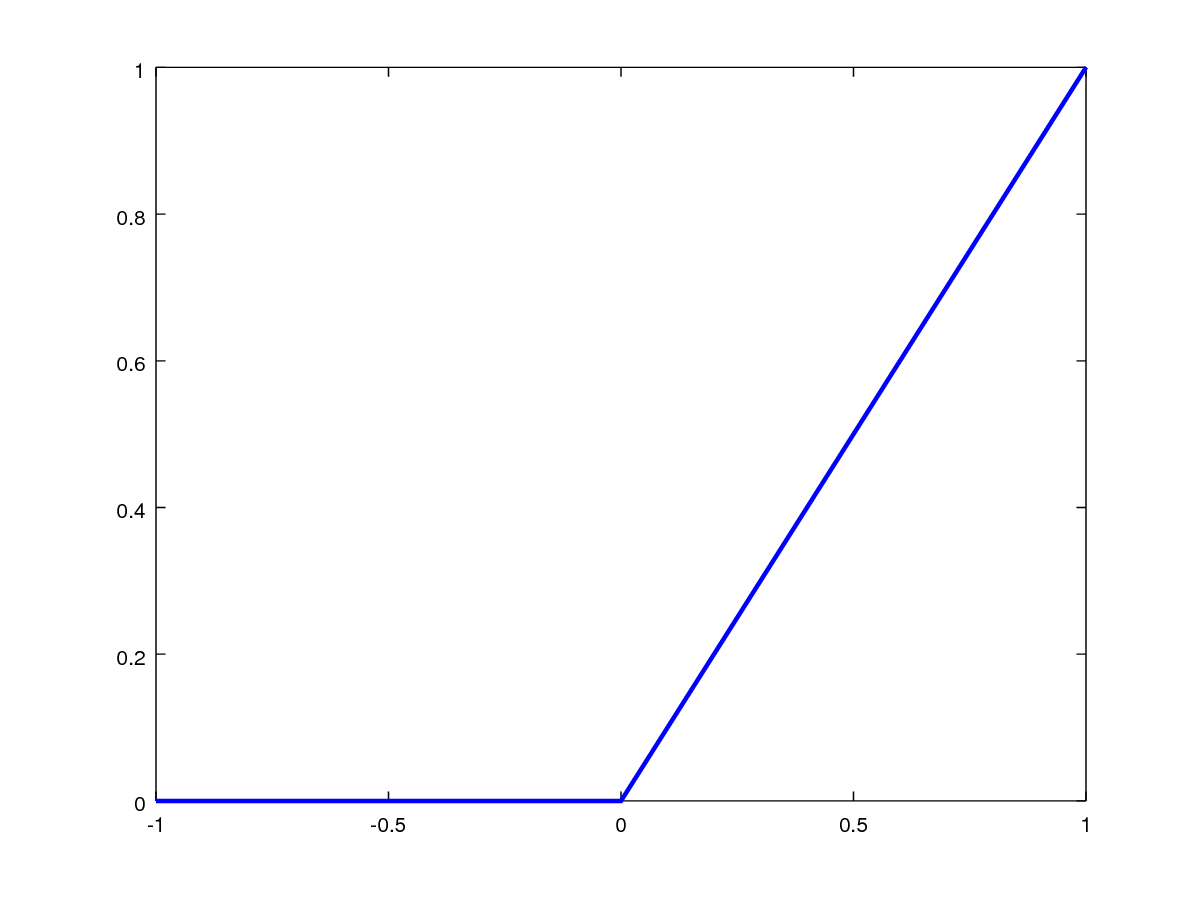
\includegraphics[width=1\linewidth]{figures/relu.png}
			\caption{\gls{relu} activation function.}\label{fig:relu}
		\end{subfigure}%
		\begin{subfigure}{0.5\textwidth}
			\centering
			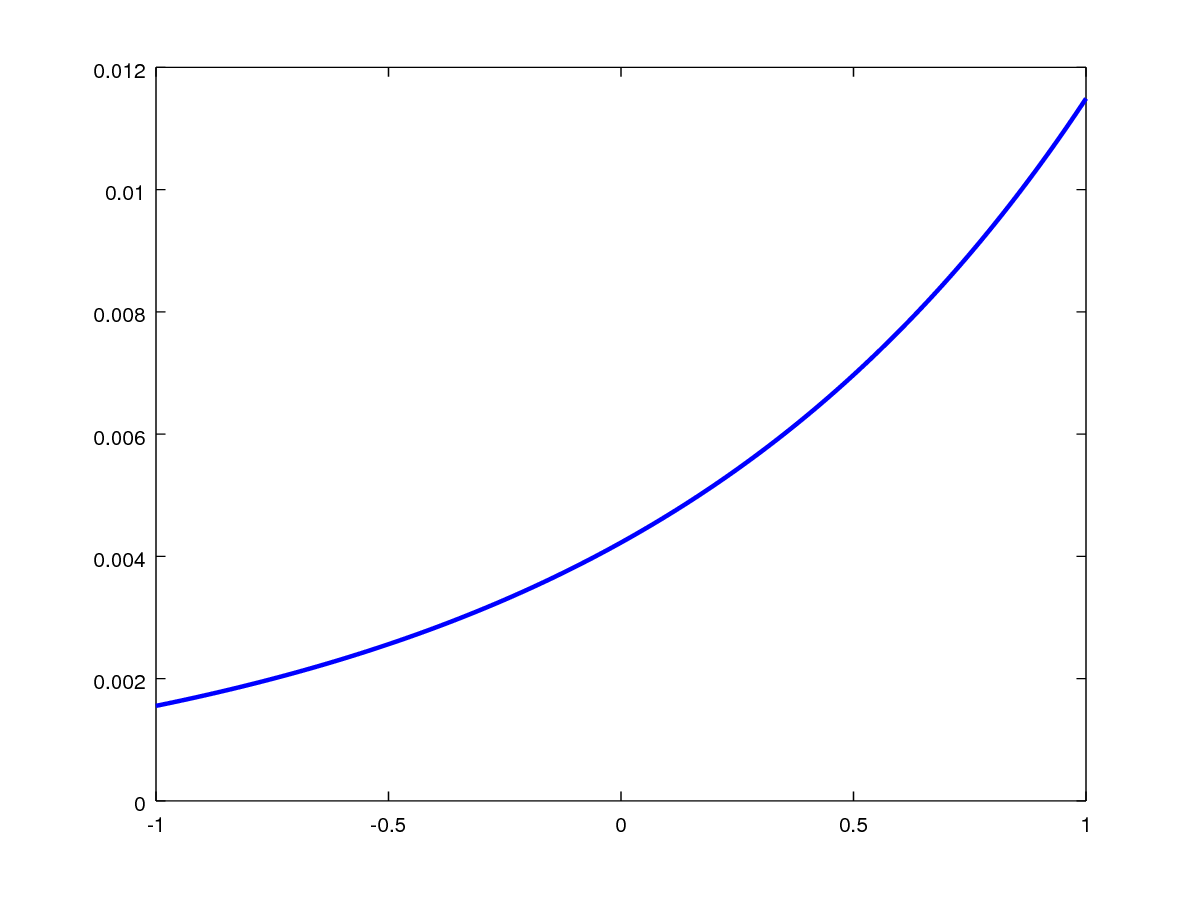
\includegraphics[width=1\linewidth]{figures/softmax.png}
			\caption{Softmax activation function.}\label{fig:softmax}
		\end{subfigure}
		\caption[Activation functions.]{}
		\label{fig:activations}
	\end{figure}
	
\end{description}

\begin{description}
	\item[Flatten layer] It \textit{flattens} the input. For instance, it converts the activation maps returned by the convolutional layers into a \textbf{vector of weights} before being connected to a dense layer. It takes no arguments.
\end{description}

\begin{description}
	\item[Dropout layer] It's considered a \textbf{regularization layer}, because its main purpose is to avoid overfitting. Dropout is a technique that randomly \textbf{\textit{switches-off}} a fraction of hidden units during training~\cite{srivastava2014dropout}. It can also be understood as a technique that "trains an ensemble consisting of all subnetworks that can be structured by removing non-output units from an underlying base network"~\cite{Goodfellow-et-al-2016}, as it can be seen in Figure~\ref{fig:dropout}.

	\begin{figure}
		\centering
		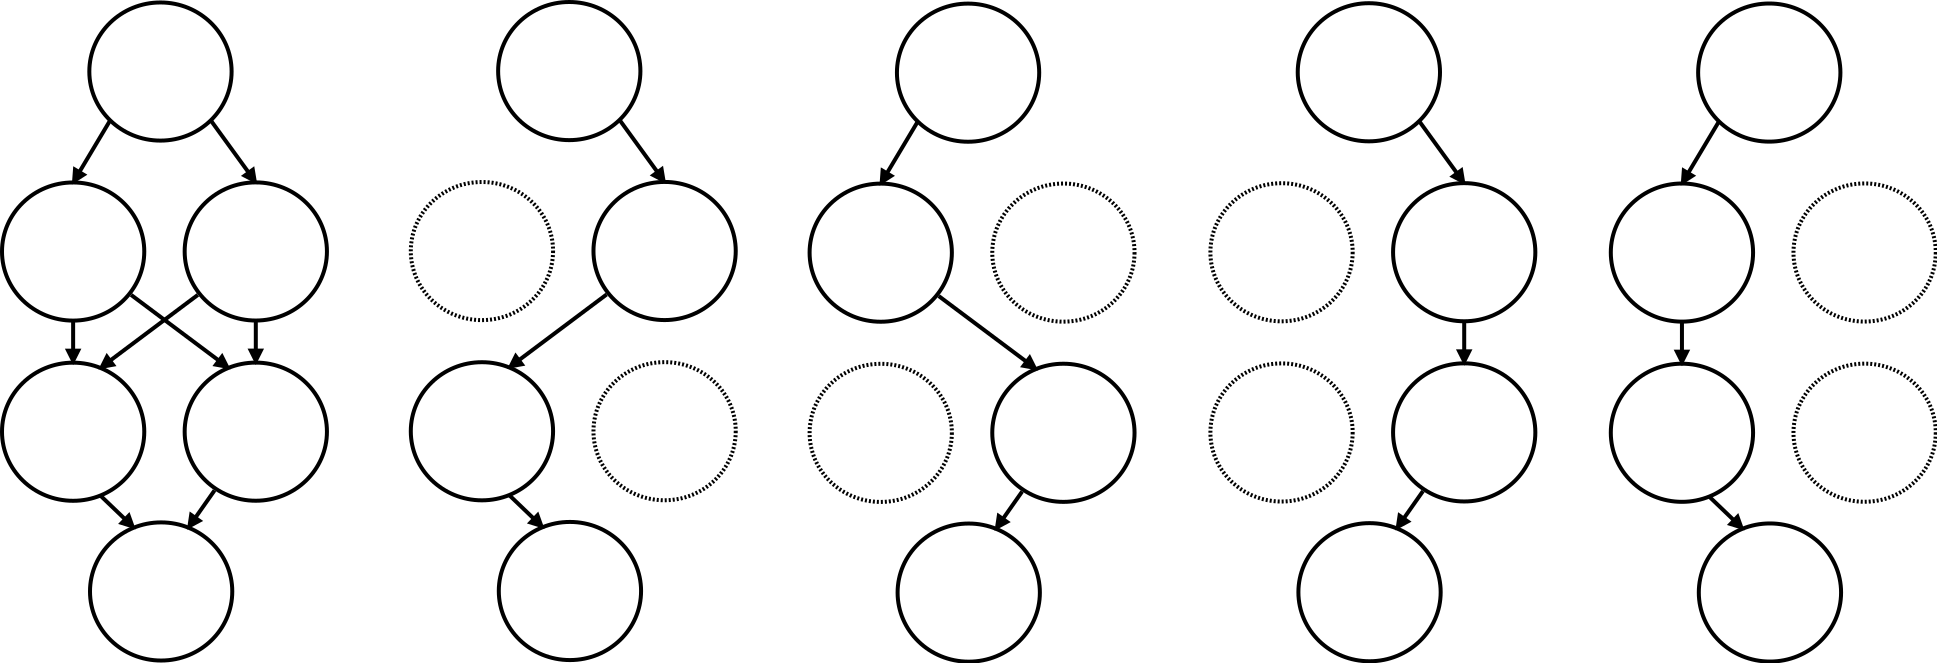
\includegraphics[width=1\linewidth, keepaspectratio]{figures/dropout.png}
		\caption{Subnetworks generated when using dropout.}
		\label{fig:dropout}
	\end{figure}	

	 This layer, as other regularization layers (i.e. GaussianNoise layer), is only active during training. It's main argument is:
	\begin{itemize}
		\item \textbf{\textit{rate}}: fraction of units that must be dropped.
	\end{itemize}
	
\end{description}

\subsection{Callbacks} \label{subsec:callbacks}
As defined by Keras documentation~\cite{chollet2015keras}, \textbf{callbacks} are a set of functions which are applied at given stages while the model is being trained. They can be used to take a look at the state of the model during training. The built-in callbacks that have been used for this project are:
\begin{itemize}
	\item \textbf{\textit{.History()}}: it is automatically applied to every Keras model and is returned by the \textit{.fit()} method. After each epoch, this callback evaluates the declared \textit{metrics} with the validation dataset and saves the results.
	
	\item \textbf{\textit{.EarlyStopping()}}: it monitors the value of a given function and forces the model to stop training when that function has stopped improving. It has a \textbf{\textit{patience}} argument which determines how many epochs in a row without improving must be tolerated before the model quits training. Setting up an appropriate \textbf{stopping criteria} may prevent the model from overfitting.
	
	\item \textbf{\textit{.ModelCheckpoint()}}: it saves the model and its weights after each epoch. It can be configured to overwrite the model only if a certain \textit{metric} has improved with respect to the previous best result, saving the best \textit{version} of it.
\end{itemize}

Additionally, Keras provides the \textit{Callback} base class that can be used to build \textbf{user-defined callbacks}.

\subsection{Image Preprocessing}\label{subsec:utils}
\textbf{Image preprocessing} is a key factor in every computer vision application. Specifically, in machine learning, besides adapting the images and extracting features before training that can improve the model performance (i.e. edge detection), it can be used to avoid \textbf{overfitting} through data augmentation. \textbf{Data augmentation}~\cite{DBLP:journals/corr/WongGSM16} consists in taking the samples that the dataset already contains and applying transformations to them, generating new samples that may be closer to real world and, in any case, enlarging the dataset with new data.

This functionality is included in Keras thanks to the \textbf{\textit{.ImageDataGenerator()} method}. It returns a batch generator which randomly applies the desired transformations to random samples of the dataset provided by the user. Built-in transformations like rotation, shifting and zooming, are passed as arguments to the aforementioned method. Additionally, it's possible to build a user-defined function and pass it as an argument as well. The dataset and the batch size are defined through the \textbf{\textit{.flow()} method}. During training, the generator will loop until the number of samples per epoch and the number of epochs set by the user are satisfied.

\subsection{Utils}
Keras include a module for multiple supplementary tasks called \textbf{\textit{Utils}}. The most important functionality for the project provided by this module is the \textbf{\textit{.HDF5Matrix()} method}. It reads the \textbf{\gls{hdf5} datasets} (see Section~\ref{sec:hdf}), which are going to be used as inputs to the neural networks.

\section{JdeRobot}\label{sec:jderobot}
\textbf{JdeRobot} is an open source middleware for robotics and computer vision~\cite{jderobot}. It has been designed to simplify the software development within these fields. It's mostly written in C\nolinebreak[4]\hspace{-.05em}\raisebox{.4ex}{\tiny\bf ++} language and it's structured like a collection of components (tools and drivers) that communicate to each other through \textbf{ICE interfaces} \footnote{\url{https://zeroc.com/products/ice}}. It is also compatible with \textbf{ROS} \footnote{\url{http://www.ros.org/}}, which allows the interoperation of ROS nodes and JdeRobot components. This flexibility makes it very useful for our application.
Its \textbf{\textit{cameraserver} driver} is going to be employed to capture images from different video sources.

\subsection*{\textit{cameraserver}}
According to JdeRobot documentation~\cite{jderobot}, this driver can serve both real cameras and video files. It communicates with other components thanks to the \textbf{\textit{Camera} interface}.

In order to use \textit{cameraserver}, its \textbf{configuration file} has to be properly set. These are the parameters that must be specified:
\begin{itemize}
	\item The \textbf{network address} where the server is going to be listening.
	
	\item Parameters related with the \textbf{video stream}: URI, frame rate, image size and format.
\end{itemize}

\section{DroidCam}\label{sec:droidcam}
On one hand, \textbf{DroidCam} is an application for Android which serves the images captured with a \textbf{smartphone camera}~\cite{droidcam}. On the other hand, it is a client for Linux which receives the video stream served by Android and makes it accessible for the computer as a \textbf{v4l2 \footnote{\url{https://www.linuxtv.org/wiki/index.php/Main_Page}} device driver}. The Linux client can be connected to the phone camera over a USB cable or a WiFi network and allows the user to control camera flash, auto-focus and zoom. DroidCam provides the address at which the Linux client must be listening to receive the images. Besides that, it provides a URL that can be used to access the video stream from any browser. 

An example of usage can be seen in Figure~\ref{fig:droidcam}. First, the Android app is opened. It shows the address where the video will be served (see Figure~\ref{fig:droidpre}). Then, the address is set in the Linux client (see Figure~\ref{fig:droidlinux}). Finally, when the \textit{Connect} button is pressed, the connection is established (see Figure~\ref{fig:droidpost})
\begin{figure}
	\centering
	\begin{subfigure}{0.33\textwidth}
		\centering
		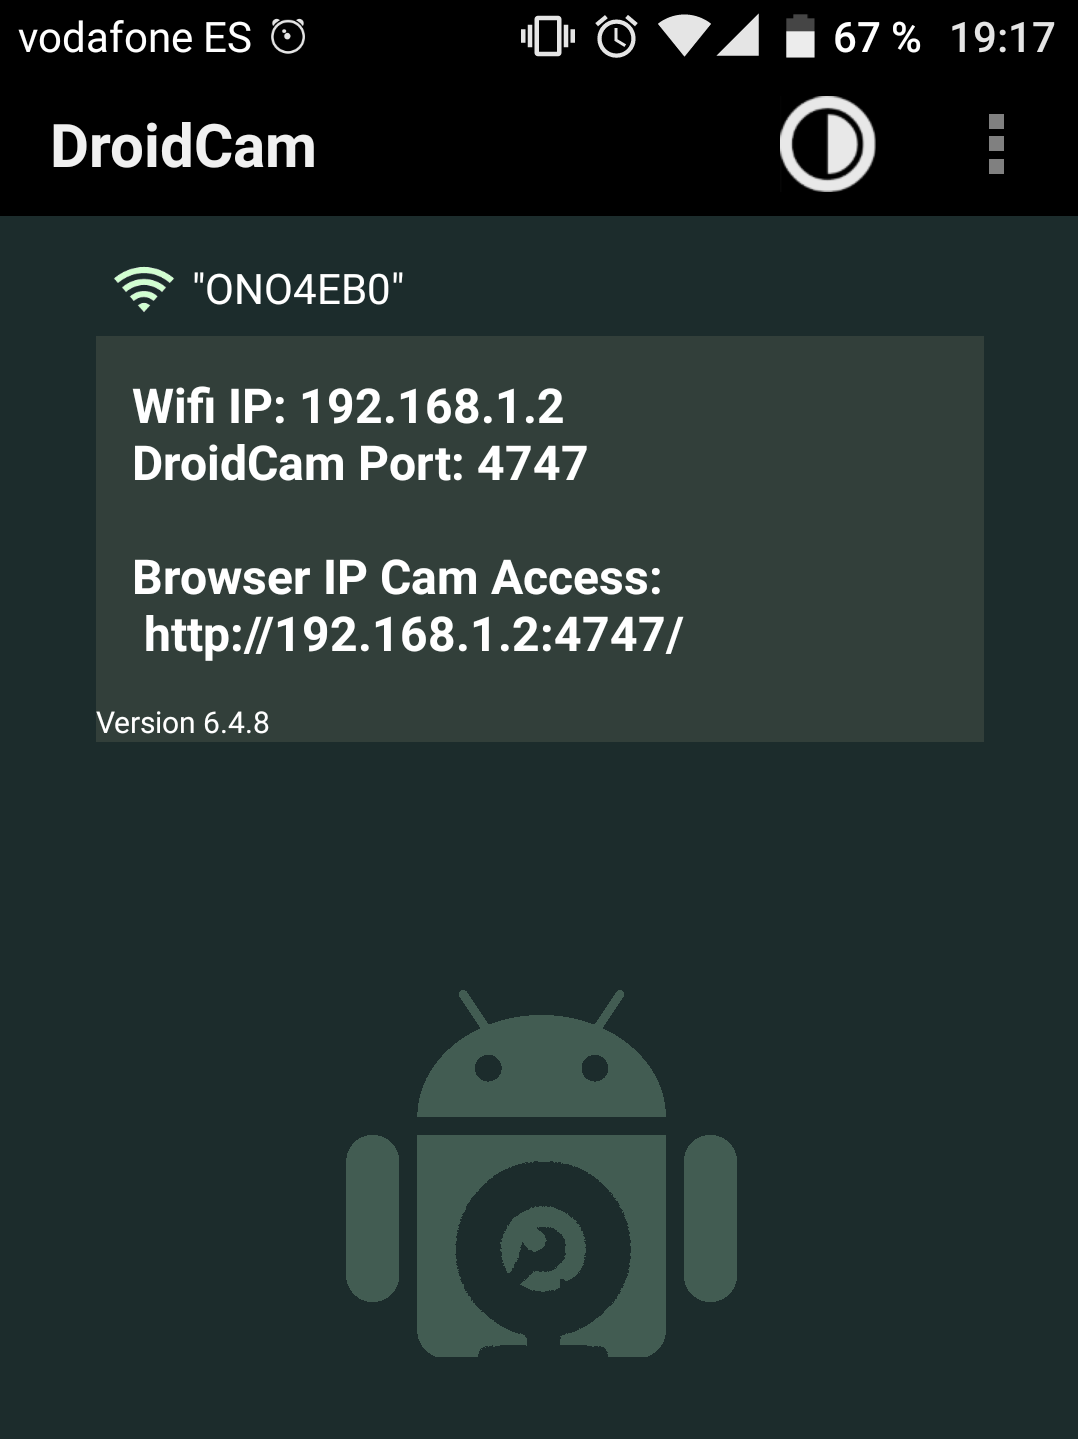
\includegraphics[width=0.9\linewidth]{figures/droidcampre.png}
		\caption{Android server.}
		\label{fig:droidpre}
	\end{subfigure}%
	\begin{subfigure}{0.33\textwidth}
		\centering
		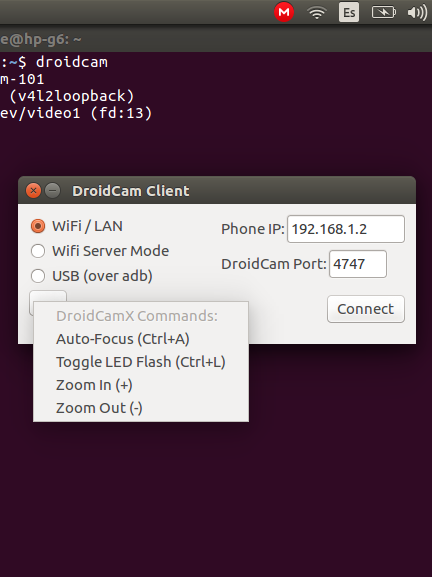
\includegraphics[width=0.9\linewidth]{figures/droidcamlinux.png}
		\caption{Linux Client.}
		\label{fig:droidlinux}
	\end{subfigure}%
	\begin{subfigure}{0.33\textwidth}
		\centering
		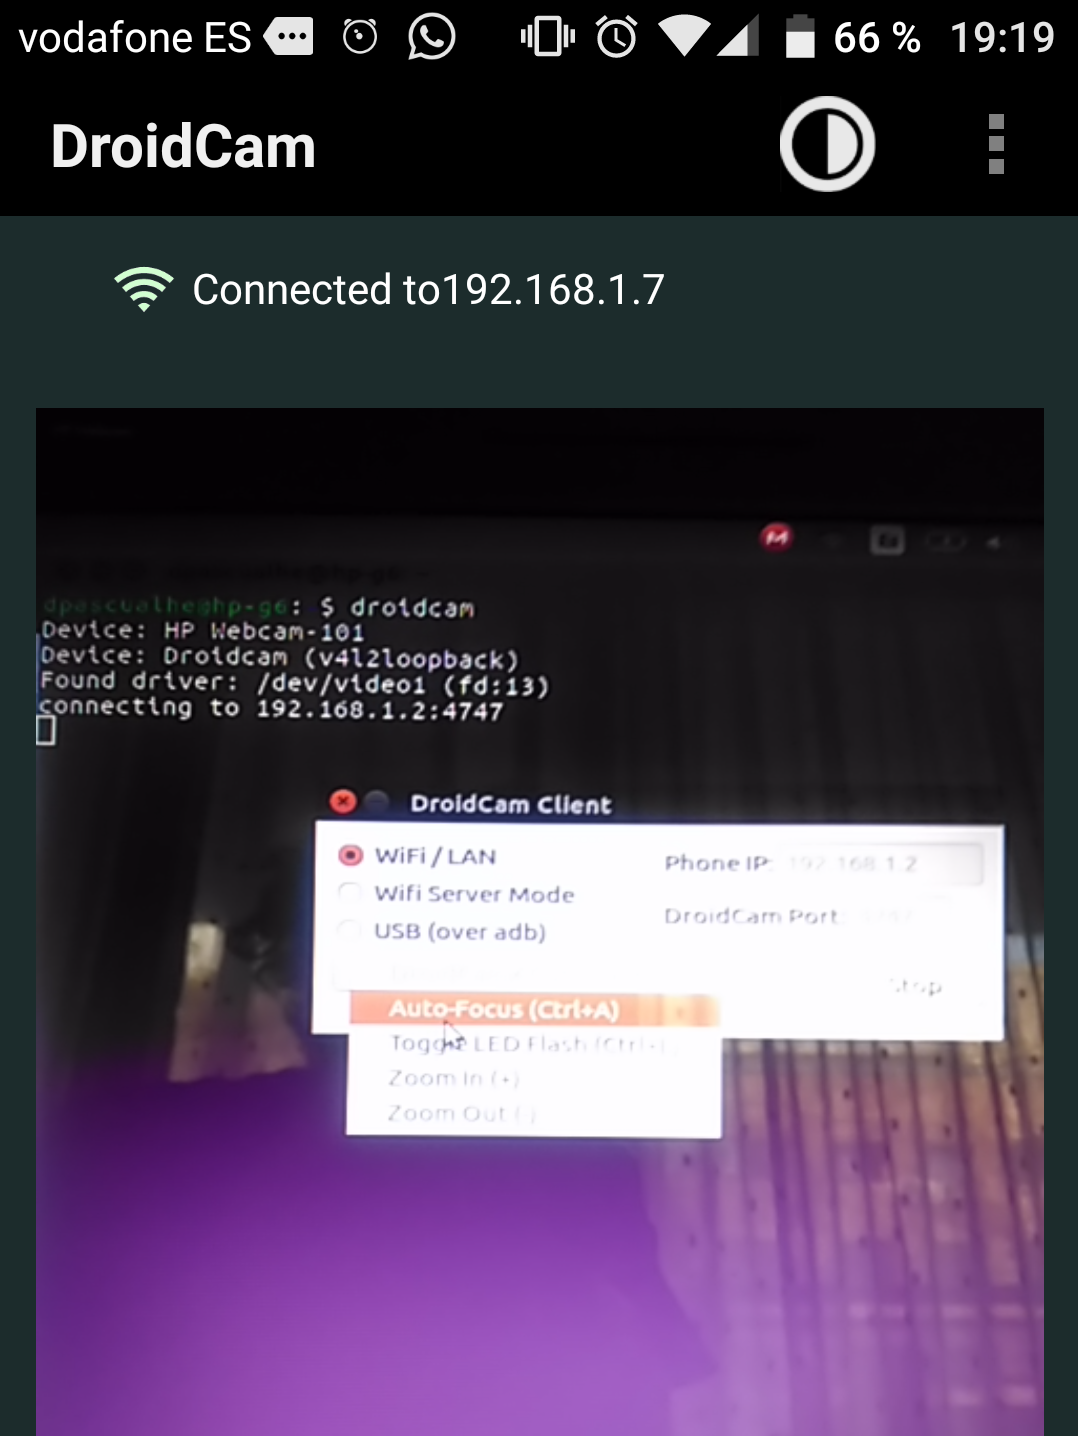
\includegraphics[width=0.9\linewidth]{figures/droidcampost.png}
		\caption{Connection established.}
		\label{fig:droidpost}
	\end{subfigure}
	\caption[DroidCam usage.]{}
	\label{fig:droidcam}
\end{figure}

\section{HDF5}\label{sec:hdf}
During the development of this project, huge amounts of data have been processed. That's why an efficient way of reading and saving this data has been an important point. Keras employs the \textbf{\gls{hdf5} file format} to save models and read datasets.

According to \gls{hdf5} documentation~\cite{hdf5}, it is a \textbf{hierarchical data format} designed for high volumes of data with complex relationships. While relational databases employ tables to store data (e.g. SQL), \gls{hdf5} supports \textbf{n-dimensional datasets} and each element in the dataset may be as complex as needed.

In order to deal with \gls{hdf5} files, the \textbf{h5py} \footnote{\url{http://www.h5py.org/}} library for Python has been employed.

\section{Scikit-learn}\label{sec:sklearn}
\textbf{Scikit-learn} is a machine learning library that includes a wide variety of algorithms for clustering, regression and classification~\cite{scikit-learn}. It can be used at every stage of the machine learning workflow: preprocessing, training, model selection and evaluation.

Scikit-learn functions have been used to evaluate the neural networks developed with Keras. Using a tool that is \textbf{independent from Keras} enables the comparison of the results achieved by different neural network libraries (e.g. Keras and Caffe). These are the evaluation parameters which have been employed in this project (equations and definitions obtained from~\cite{scikit-doc}):
\begin{itemize}
	\item \textbf{Precision}: ability of the classifier not to label as positive a sample that is negative.
	\begin{equation}\label{eq:precision}
	\textrm{precision}=\frac{true_{positives}}{true_{positives}+false_{positives}}
	\end{equation}
	
	\item \textbf{Recall}: ability of the classifier to find all the positive samples.
	\begin{equation}\label{eq:recall}
	\textrm{recall}=\frac{true_{positives}}{true_{positives}+false_{negatives}}
	\end{equation}
	
	\item \textbf{Confusion matrix}: a matrix where the element $i,j$ represents the number of samples that belongs to the group $i$ but has been classified as belonging to group $j$. True predictions can be found in the diagonal of the matrix, where $i=j$. An example of a confusion matrix constructed with Scikit-learn and displayed with Octave (see Section~\ref{sec:octave}) can be found in Figure~\ref{fig:conf_mat}.
\end{itemize}

Besides the functions that have just been mentioned, \textbf{accuracy} and \textbf{log loss} have also been used and they're defined as in Section~\ref{subsec:models}.

\section{Octave} \label{sec:octave}
\textbf{GNU Octave}~\cite{octave} is a scientific programming language compatible with \textbf{Matlab}. It provides powerful tools for plotting, which have been used to visualize the data collected with Scikit-learn about the performance of the models. An example of Octave usage can be seen in Figure~\ref{fig:conf_mat}.
\begin{figure}
	\centering
	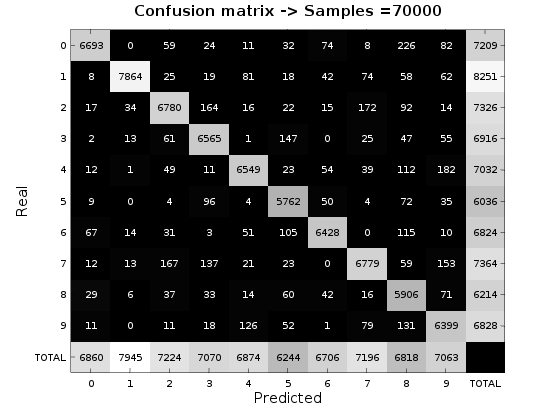
\includegraphics[width=0.8\linewidth, keepaspectratio]{figures/conf_mat.png}
	\caption{Example of a confusion matrix visualization using Octave.}
	\label{fig:conf_mat}
\end{figure}
\lhead[]{CHAPTER \thechapter. DIGIT CLASSIFIER}
\chapter{Digit classifier}\label{ch:digitclass}
Taking advantage of the \glspl{cnn} impressive performance in classification tasks, we have built a \emph{real-time digit classifier}. Its core elements are:
\begin{itemize}
	\item A \emph{Keras model} (see Section~\ref{subsec:models}), which classifies the images.
	\item A \emph{JdeRobot component}, which acquires and processes the images from a video stream and integrates a Keras model to classify them. The images and the classification results are displayed within a \gls{gui}.
\end{itemize}

\section{Understanding the Keras model}\label{sec:understanding}
Understanding how Keras models work is a key factor in the development of this project. For this purpose, an adapted version of an example provided by Keras\footnote{\url{https://git.io/vH0qw}} will be analyzed in the following sections. In this example, a \gls{cnn} is trained and tested with the \emph{\gls{mnist} database} of handwritten digits (see Section~\ref{sec:datasets}).

\subsection{Adapting data}\label{subsec:adaptdata}
First of all, the input data have to be loaded and adapted. Keras library contains a module named \textit{datasets} from which a variety of databases can be imported, including \gls{mnist}. The \gls{mnist} database can be loaded calling the \textit{mnist.load\_data()} method. It returns, as \emph{Numpy arrays}, the images and labels from both training and test datasets, as it is shown in the code below, which also displays the first sample of the \gls{mnist} training dataset (see Figure~\ref{fig:firstsample}).
\begin{lstlisting}
(x_train, y_train), (x_test, y_test) = mnist.load_data()

cv2.imshow('First sample',x_train[0])
cv2.waitKey(5000)
cv2.destroyWindow('First sample')

print ('Original input images data shape: ', x_train.shape) 
\end{lstlisting}

That code also prints the shape of the dataset:
\begin{Verbatim}[frame=single]
Original input images data shape:  (60000, 28, 28)
\end{Verbatim}

\begin{figure}
	\centering
	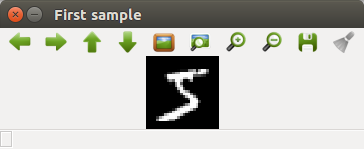
\includegraphics[width=0.7\linewidth, keepaspectratio]{figures/first_sample.png}
	\caption{First sample of the MNIST database.}
	\label{fig:firstsample}
\end{figure}

According to that, the training dataset includes~60000~images, each one containing~28x28~pixels. In order to feed the Keras model, the number of channels of the samples have to be explicitly declared, so the dataset must be \emph{reshaped}. In this case, the samples are \emph{grayscale images}, which implies that the number of channels is equal to 1. For instance, if they had been RGB images, the number of channels would have been equal to 3. As data are stored in Numpy arrays, it can be reshaped using the \textit{.reshape()} method. The order in which dimensions must be declared depends on the \textit{.image\_dim\_ordering()} parameter of the Keras \textit{backend}, as it is shown in the following code.
\begin{lstlisting}
img_rows, img_cols = 28, 28
...
if backend.image_dim_ordering() == 'th':
	# reshapes 3D data provided (nb_samples, width, height) into 4D
	# (nb_samples, nb_features, width, height) 
	x_train = x_train.reshape (x_train.shape[0], 1, img_rows, img_cols)
	x_test = x_test.reshape (x_test.shape[0], 1, img_rows, img_cols)
	input_shape = (1,img_rows,img_cols)
	print ('Input images data reshaped: ', (x_train.shape))
	print ('--------------------------------------------------------------')
else:
	# reshapes 3D data provided (nb_samples, width, height) into 4D
	# (nb_samples, nb_features, width, height) 
	x_train = x_train.reshape(x_train.shape[0], img_rows, img_cols, 1)
	x_test = x_test.reshape(x_test.shape[0], img_rows, img_cols, 1)
	input_shape = (img_rows, img_cols, 1)
	print ('Input images data reshaped: ', (x_train.shape))
	print ('--------------------------------------------------------------')
\end{lstlisting}

In this case, the training dataset gets reshaped as follows:
\begin{Verbatim}[frame=single]
Input images data reshaped:  (60000, 28, 28, 1)
\end{Verbatim}

The last step to get the input images ready is to convert \emph{data type} from \textit{uint8} to \textit{float32} and normalize pixel values to $[0,1]$ range:
\begin{lstlisting}
print('Input images type: ',x_train.dtype)
x_train = x_train.astype('float32')
x_test = x_test.astype('float32')
print('New input images type: ',x_train.dtype)
print ('-----------------------------------------------------------------')
x_train /= 255
x_test /= 255
\end{lstlisting}

Regarding the \emph{labels}, they are originally shaped as an array in which each element is an integer in the range $[0, 9]$. In other words, each element contains the digit that corresponds to a certain sample. In order to feed the Keras model, labels have to be reshaped into \emph{probability distributions}, that is, an array in which each element represents the probability of occurrence of each digit. For example, if the element of the original array is 2, in the reshaped array it will be $[0, 0, 1, 0, 0, 0, 0, 0, 0, 0]$. This conversion is achieved using the Keras built-in method \emph{\textit{np\_utils.to\_categorical()}}:
\begin{lstlisting}
nb_classes = 10
...
print ('First 10 class labels: ', (y_train[:10]))
print ('Original class label data shape: ', (y_train.shape))
# converts class vector (integers from 0 to nb_classes) to class matrix
# (nb_samples, nb_classes)
y_train = np_utils.to_categorical(y_train, nb_classes)
y_test = np_utils.to_categorical(y_test, nb_classes)
print ('Class label data reshaped: ', (y_train.shape))
print ('-----------------------------------------------------------------')
\end{lstlisting}

That code prints:
\begin{Verbatim}[frame=single]
First 10 class labels:  [5 0 4 1 9 2 1 3 1 4]
Original class label data shape:  (60000,)
Class label data reshaped:  (60000, 10)
\end{Verbatim}

\subsection{Model architecture}
Once data are ready, the \gls{cnn} architecture must be defined. In this example, a \emph{sequential model} (see Section~\ref{subsec:models}) is enough for solving the classification task and it is declared as follows:
\begin{lstlisting}
model = Sequential()
\end{lstlisting}

The next step is to add the corresponding layers. The core layers of a \gls{cnn}, as treated by Keras, have been already defined in Section~\ref{subsec:layers}. The following code performs the addition of the layers to the model.
\begin{lstlisting}
nb_filters = 32
kernel_size = (3, 3)
pool_size = (2, 2)
...
# convolutional layer
model.add(Convolution2D(nb_filters, kernel_size[0], kernel_size[1],
                          border_mode='valid', input_shape=input_shape, 
                          activation='relu'))
# convolutional layer
model.add(Convolution2D(nb_filters, kernel_size[0], kernel_size[1],
                          activation='relu'))
# pooling layer
model.add(MaxPooling2D(pool_size=pool_size))
# dropout layer
model.add(Dropout(0.25))
# flattening the weights (making them 1D) to enter fully connected layer
model.add(Flatten())
# fully connected layer
model.add(Dense(128, activation='relu'))
# dropout layer to prevent overfitting
model.add(Dropout(0.5))
# output layer
model.add(Dense(nb_classes, activation='softmax'))
\end{lstlisting}

As defined by the code above, the model is formed by the following layers:
\begin{itemize}
	\item A \emph{2D convolutional layer} with~32~filters of size~3x3x1.
	\begin{itemize}
		\item Since this is the first layer of the model, the \emph{\textit{input\_shape}} argument must be provided. In this case, the input shape is~28x28x1. 
		\item As \textit{valid} mode is set, \emph{no padding} is applied and the output dimension will be reduced. 
		\item \emph{\gls{relu} activation function} (see Equation~\ref{eq:relu}) introduces non-linearity into the network. If the activation functions were linear, the whole stack of layers could be reduced to a single layer, losing much of the ability to learn different levels of features.
		\item This layer outputs~32~activation maps with size~26x26.
	\end{itemize}
	
	\item Another \emph{convolutional layer} with the same arguments:~32~filters, no padding and \gls{relu} as activation function.
	\begin{itemize}
		\item Increasing the number of convolutional layers allows the \gls{cnn} to learn \emph{more complex features}. 
		\item As the depth of its input is~32~(one channel per activation map), the size of the filters will be~3x3x32. 
		\item This layer outputs~32~activation maps with size~24x24.
	\end{itemize}
	
	\item A \emph{2D MaxPooling layer} with a \textit{pool\_size} of~2x2.
	\begin{itemize}
		\item This layer outputs the~32~activation maps generated by the previous layer, but \emph{\textit{downsampled}} by a factor of~2, resulting in maps with size~12x12.
	\end{itemize}
	
	\item A \emph{dropout layer} to prevent overfitting. 
	\begin{itemize}
		\item The fraction of random units that are going to be \emph{\textit{swicthed-off}} is~0.25.
		\item This layer preserves the size and the shape of its input.
	\end{itemize} 
	
	\item A \emph{flatten layer} that turns the matrices of weights that it receives into a vector that can be fed to the fully-connected layer.
	\item A fully-connected or \emph{dense layer}.
	\begin{itemize}
		\item This layer contains~128~neurons that will output an array of~128~values.
		\item Once more, the \emph{\gls{relu} activation function} is applied.
	\end{itemize} 
	
	\item A \emph{dropout layer} with a~0.5~fraction.
	
	\item Finally, the \emph{output layer} is another \emph{dense layer} which contains as many neurons as classes, in this example,~10. 
	\begin{itemize}
		\item In order to output a \emph{probability distribution} of the predicted classes, the activation function will be \emph{softmax} (Equation~\ref{eq:SoftMax}).
	\end{itemize}
\end{itemize}

The resulting architecture and data shape after every layer are shown in Figure~\ref{fig:model}.

\begin{figure}
	\centering
	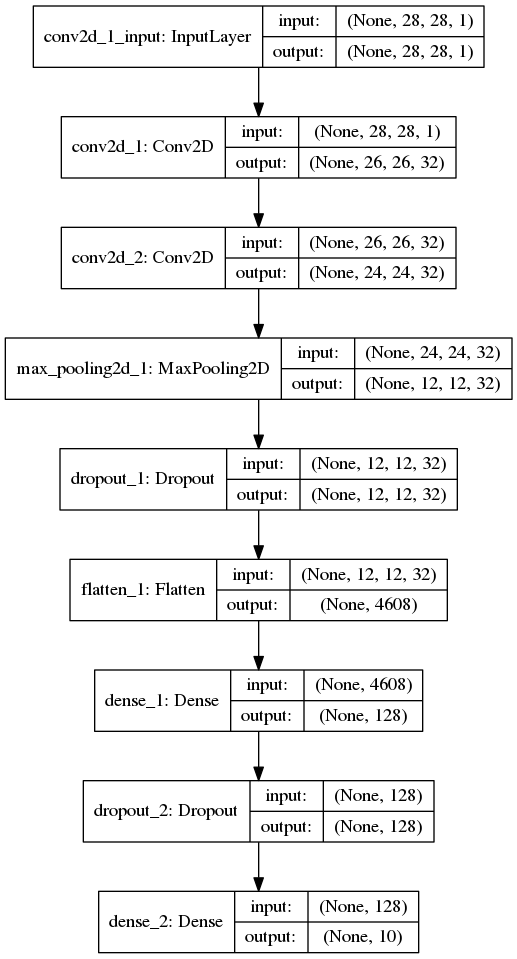
\includegraphics[width=0.6\linewidth, keepaspectratio]{figures/model.png}
	\caption{Diagram of a Keras sequential model.}
	\label{fig:model}
\end{figure}

\subsection{Compiling the model}
After declaring the model and defining its architecture, the \emph{learning process} must be set through the  \textit{.compile()} method. The arguments required to set this process are defined in Section~\ref{subsec:models}. The code can be seen in the next frame:
\begin{lstlisting}
model.compile(loss='categorical_crossentropy', optimizer='adadelta', 
               metrics=['accuracy'])
\end{lstlisting}

In this example, the loss function that is computed after every batch is the \emph{categorical cross-entropy} (see Equation~\ref{eq:categorical_crossentropy}) and the optimizer that updates the weights of the \gls{cnn} in order to minimize that loss function is \emph{ADADELTA}. Additionally, the \emph{accuracy} is also computed to monitor the \gls{cnn} performance during training.

\subsection{Training the model}
The \gls{cnn} is trained thanks to the \textit{.fit()} method, which has been already described in Section~\ref{subsec:models}. The usage of that method can be seen in the code below.
\begin{lstlisting}
nb_epoch = 12
batch_size = 128
...
model.fit(x_train, y_train, batch_size=batch_size, nb_epoch=nb_epoch,
           verbose=1, validation_data=(x_test, y_test))
\end{lstlisting}

The model will be trained for~12~\emph{epochs} and the \emph{batch size}, i.e. the number of samples that pass through the \gls{cnn} before updating the weights, is~128. The test dataset is used here as \emph{validation data}, for which the log loss and the accuracy will be computed after every epoch just for \emph{monitoring purposes}. During training time, Keras prints the results after every batch and epoch as follows:
\begin{Verbatim}[frame=single]
Train on 60000 samples, validate on 10000 samples
Epoch 1/12
128/60000 [....................] - ETA: 350s - loss: 2.3223 - acc: 0.1016
256/60000 [....................] - ETA: 312s - loss: 2.3073 - acc: 0.1094
...
59776/60000 [==================>.] - ETA: 1s - loss: 0.0455 - acc: 0.9871
59904/60000 [==================>.] - ETA: 0s - loss: 0.0455 - acc: 0.9871
60000/60000 [====================] - 407s - loss: 0.0455 - acc: 0.9871 - 
val_loss: 0.0306 - val_acc: 0.9891
\end{Verbatim}

\subsection{Testing the model}
Once the model is trained, its weights, architecture and learning configuration can be stored in an \emph{\gls{hdf5} file} (see Section~\ref{sec:hdf}). Besides that, in order to see the performance of the \gls{cnn}, the \textit{.evaluate()} method takes the test dataset and computes the \emph{log loss} and the \emph{accuracy}, as it is shown in the following code:
\begin{lstlisting}
model.save('MNIST_net.h5')

score = model.evaluate(x_test, y_test, verbose=0)
print('Test score:', score[0])
print('Test accuracy:', score[1])
\end{lstlisting}
These are the results obtained with this example (\textit{Test score} refers to loss):
\begin{Verbatim}[frame=single]
Test score: 0.0306129640532
Test accuracy: 0.9891
\end{Verbatim}

\section{JdeRobot component}\label{sec:component}
Once the \gls{cnn} has been trained and the resultant model is saved, the next milestone is to integrate it into a JdeRobot component that must be able to acquire images from a video stream, apply the necessary preprocessing and display the predictions obtained from them. That component is \emph{\textit{digitclassifier.py}} and it is based on Nuria Oyaga's code\footnote{\url{https://github.com/RoboticsURJC-students/2016-tfg-nuria-oyaga}}. Figure~\ref{fig:digitclass} shows the program running.

\begin{figure}
	\centering
	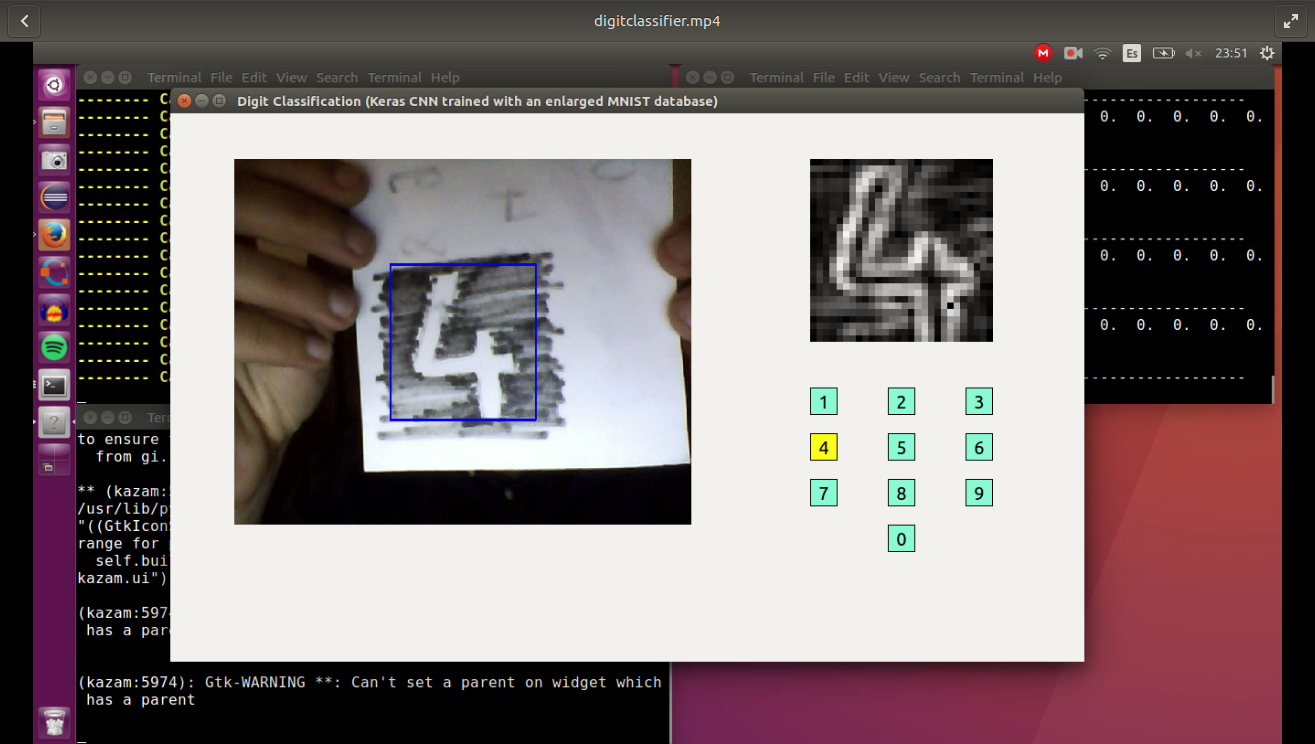
\includegraphics[width=1\linewidth, keepaspectratio]{figures/digitclass.png}
	\caption{Example of \textit{digitclassifier.py} execution.}
	\label{fig:digitclass}
\end{figure}

\subsection{Design}
Before analyzing in detail the internals of the digit classifier component, its design will be described. For this purpose, the \emph{block diagrams} shown in Figure~\ref{fig:dia} have been built.

Figure~\ref{fig:dia}(a) shows a \emph{high-level diagram} of the process followed from the video source to the predicted digit. First, images captured with the camera are received by the \emph{cameraserver} driver. Then, the digit classifier component communicates with this driver and gets the images. Finally, a prediction is made. Optionally, if images are captured with a smartphone camera, DroidCam can receive those images and create a camera device that can communicate with the \emph{cameraserver} driver.

In Figure~\ref{fig:dia}(b), the  \emph{internals of the digit classifier component} are shown. The main program (\emph{digitclassifier.py}) starts two threads, \textit{ThreadCamera} and \textit{ThreadGUI}. These threads update \textit{GUI} and \textit{Camera} classes concurrently. \textit{Camera} class communicates with \textit{cameraserver} to get the images, which are then preprocessed. The preprocessed image is fed to the Keras model and a prediction is made. Original and preprocessed images, as well as the predicted digits, are passed to the \textit{GUI} class, which displays all of them in the screen.
\begin{figure}
	\begin{subfigure}{1\textwidth}
		\centering
		\includegraphics[width=0.8\linewidth]{figures/diagram_black.png}
		\caption{}
	\end{subfigure}
	\begin{subfigure}{1\textwidth}
		\centering
		\includegraphics[width=0.8\linewidth]{figures/diagram_transparent.png}
		\caption{}
	\end{subfigure}
	\caption{Digit classifier design: (a) high-level; (b) lower-level.}
	\label{fig:dia}
\end{figure}

\subsection{\textit{Camera} class}
\emph{\textit{Camera} class} is responsible for getting the images, transforming them into a suitable input for the Keras model and returning the classification results.

\begin{itemize}
	\item \textbf{Acquisition}. The images are served by the JdeRobot component \emph{\textit{cameraserver}} (see Section~\ref{sec:jderobot}). Depending on how its configuration file (\textit{cameraserver.cfg}) has been set, the images can come from different kinds of video streams. Connection with \emph{webcams} and \emph{video files} is straightforward: the URI property in the configuration file must be changed to the number of device or the path of the video, as it is shown in the code below.
	\begin{lstlisting}[frame=single]
	#0 corresponds to /dev/video0, 1 to /dev/video1, and so on...
	#CameraSrv.Camera.0.Uri=1                                # webcam
	CameraSrv.Camera.0.Uri=/home/dpascualhe/video.mp4        # video file
	\end{lstlisting}
	
	In order to establish a connection with smartphone cameras, the \emph{DroidCam application} for Android has been used (see Section~\ref{sec:droidcam}). As this application turns the video stream provided by the smartphone into a \emph{v4l2\footnote{\url{https://www.linuxtv.org/wiki/index.php/Main_Page}} device driver}, the video stream will be listed as another webcam and the number of device must be set in the \textit{cameraserver} configuration file.
	
	Besides that, the \emph{address} at which the video is being served by the \textit{cameraserver} component must be provided to the \textit{Camera} class through another configuration file: \emph{\textit{digitclassifier.cfg}}.
	
	\item \textbf{Preprocessing}. As images can be captured with different devices, the \textit{digitclassifier.py} component must apply some preprocessing that mitigates the differences between video streams and that makes the images suitable for the Keras model. The following \emph{transformations} are applied before classification:
	\begin{enumerate}
		\item Images are \emph{cropped} into~80x80~pixels images. The \emph{\gls{roi}} from which cropped images are extracted is draw over the original image, making it easier to aim at digits with the camera.
		\item Color doesn't provide any useful information about digits and \gls{mnist} database is formed by \emph{grayscale images}. For this reason, the images captured with the component are converted into grayscale images as well. 
		\item A \emph{Gaussian filtering} is applied in order to reduce image \emph{noise}. When using this operator, the \emph{kernel size} and the \emph{standard deviation} $\sigma$ in $x$ and $y$ should be specified~\cite{itseez2014theopencv}. In this case, the kernel size will be~5x5~and the standard deviation is automatically calculated depending on that size. The 2D Gaussian filter, as defined in~\cite{sonka1999image}, is given by:
		\begin{equation}
		G(x,y)=\exp(-\frac{x^2+y^2}{2\sigma^2})
		\end{equation}
		\item After reducing noise, the image is \emph{resized} to fit the Keras \emph{model input}. The new size is~28x28~pixels, like \gls{mnist} samples.
		\item Last step is obtaining the \emph{gradient of the images}. Working with this kind of images instead of the original ones allows the application to deal with different light and color conditions. The chosen algorithm for this task is \emph{Sobel filter} (Equation~\ref{eq:sobel}). This will be deeply discussed in Section~\ref{subsec:edge}.
	\end{enumerate}
	
	The following code applies the transformations mentioned above:
\begin{lstlisting}[frame=single]
def trasformImage(self, im):
''' Transforms the image into a 28x28 pixel grayscale image and
applies a sobel filter (both x and y directions).
''' 
	im_crop = im [140:340, 220:420]
	im_gray = cv2.cvtColor(im_crop, cv2.COLOR_BGR2GRAY)
	im_blur = cv2.GaussianBlur(im_gray, (5, 5), 0) # Noise reduction.
	
	im_res = cv2.resize(im_blur, (28, 28))
	
	# Edge extraction.
	im_sobel_x = cv2.Sobel(im_res, cv2.CV_32F, 1, 0, ksize=5)
	im_sobel_y = cv2.Sobel(im_res, cv2.CV_32F, 0, 1, ksize=5)
	im_edges = cv2.add(abs(im_sobel_x), abs(im_sobel_y))
	im_edges = cv2.normalize(im_edges, None, 0, 255, cv2.NORM_MINMAX)
	im_edges = np.uint8(im_edges)
	
	return im_edges
\end{lstlisting}
	
	\item \textbf{Classification}. Before entering the \gls{cnn}, the images are \emph{reshaped} as mentioned in Section~\ref{subsec:adaptdata}. \textit{Camera} class calls Keras \emph{\textit{.predict()} method} (see Section~\ref{subsec:models}) to get the predicted digit. The prediction is only taken into account if one of the probabilities is equal to 1, avoiding wrong answers when the prediction is not clear. The function that performs the classification can be seen in the following frame:
\begin{lstlisting}
def classification(self, im):
''' Adapts image shape depending on Keras backend (TensorFlow
or Theano) and returns a prediction.
'''
	if backend.image_dim_ordering() == 'th':
		im = im.reshape(1, 1, im.shape[0], im.shape[1])            
	else:      
		im = im.reshape(1, im.shape[0], im.shape[1], 1)            
	
	dgt = np.where(self.model.predict(im) == 1)
	if dgt[1].size == 1:
		self.digito = dgt
	else:
		self.digito = (([0]), (["none"]))
	
	return self.digito[1][0]
\end{lstlisting}
\end{itemize}

\subsection{\textit{GUI} class}
\emph{\textit{GUI} class} displays the original image, the preprocessed image and the result of the classification, as it is shown in Figure~\ref{fig:digitclass}. It has been built employing the \emph{pyQt package}\footnote{\url{https://pypi.python.org/pypi/PyQt4}}\footnote{\url{https://pypi.python.org/pypi/PyQt5}}. It is based in Nuria Oyaga's code, but it has been updated from Qt4 to Qt5 thanks to the information provided by PyQT documentation~\cite{pyqt5}.

\subsection{Threads} 
In order to capture images and update the \gls{gui} concurrently, the \emph{\textit{threading} module}~\cite{threading}, provided by Python, has been employed. From this module, a subclass of the \emph{\textit{Thread} object} is created. In this new subclass, \textit{\_\_init\_\_()} and \textit{.run()} methods are overriden. The \textit{.run()} method will be responsible for calling a process that updates the thread. For example, the \textit{.update()} method of the \textit{Camera} class, which reads a new image from the video stream each time it is invoked, is called within the \textit{.run()} method of the \emph{\textit{ThreadCamera} class}. Besides that, in the \textit{.run()} method, the \emph{cycle time} is adjusted. The next frame shows how the \textit{ThreadCamera} class is coded:
\begin{lstlisting}
import time
import threading
from datetime import datetime

t_cycle = 150  # ms

class ThreadCamera(threading.Thread):

def __init__(self, cam):
''' Threading class for Camera. '''
	self.cam = cam
	threading.Thread.__init__(self)

def run(self):
''' Updates the thread. '''
	while(True):
		start_time = datetime.now()
		self.cam.update()
		end_time = datetime.now()
		
		dt = end_time - start_time
		dtms = ((dt.days * 24 * 60 * 60 + dt.seconds) * 1000
		+ dt.microseconds / 1000.0)
		
		if(dtms < t_cycle):
			time.sleep((t_cycle - dtms) / 1000.0);
\end{lstlisting}

\subsection{Main program}
All of these elements are joined together in \emph{\textit{digitclassifier.py}}. \textit{Camera}, \textit{GUI} and their threads are initialized and the \textit{.start()} methods of the \textit{Thread} objects are invoked, as it is shown in the code below:
\begin{lstlisting}
if __name__ == '__main__':

cam = Camera()
app = QtWidgets.QApplication(sys.argv)
window = GUI()
window.setCamera(cam)
window.show()

# Threading camera
t_cam = ThreadCamera(cam)
t_cam.start()

# Threading GUI
t_gui = ThreadGUI(window)
t_gui.start()

sys.exit(app.exec_())
\end{lstlisting}

In order to execute the program:
\begin{enumerate}
	\item \textit{cameraserver} must be launched with its configuration file as an argument in a terminal:
	\begin{Verbatim}[frame=single]
dpascualhe@hp-g6:~$ cameraserver cameraserver.cfg
	\end{Verbatim}
	
	\item In another terminal, \textit{digitclassifier.py} must be launched with its configuration file as well:
	\begin{Verbatim}[frame=single]
dpascualhe@hp-g6:~$ python digitclassifier.py digitclassifier.cfg
	\end{Verbatim}
\end{enumerate}

An example of usage of the digit classifier component can be seen in Figure~\ref{fig:digitclass}.

\lhead[]{CHAPTER \thechapter. BENCHMARK}
\chapter{Benchmark}\label{ch:benchmark}
The model described in Section~\ref{sec:understanding} can be improved with different architectures and regularization methods. Besides that, training the model with new datasets can also lead to better results. In order to \textbf{compare the performance} of these new models, a \textbf{benchmark} has been established. In this chapter, the datasets employed to train the models, as well as the tools developed to measure and visualize their performance will be described.

\section{Datasets}\label{sec:datasets}
The digit classifier component is possible thanks to the data provided by the \textbf{\gls{mnist} database} of handwritten digits. In the following sections, the pros and cons of using this database and some alternatives will be discussed.

\subsection{Original dataset}\label{subsec:MNIST}
\textbf{\gls{mnist}} is a database of \textbf{handwritten digits} formed by a training set, which contains~60000~samples, and a test set, containing~10000~samples~\cite{lecun-mnisthandwrittendigit-2010}. It's a \textit{remixed} and reduced version of the original \textbf{NIST datasets} \footnote{\url{https://www.nist.gov/srd/nist-special-database-19}}. \gls{mnist} is a well-known benchmark for all kinds of machine learning algorithms.

As may be seen in Figure~\ref{fig:mnist}, each sample of the \gls{mnist} database is a~28x28~pixels \textbf{grayscale image} that contains a size-normalized and centered digit. While it may be useful for testing machine learning algorithms, it's not enough to train a model that aims to solve a \textbf{real-world task}, because the images are almost noiseless and share similar orientation, position, size and intensity levels.
\begin{figure}
	\centering
	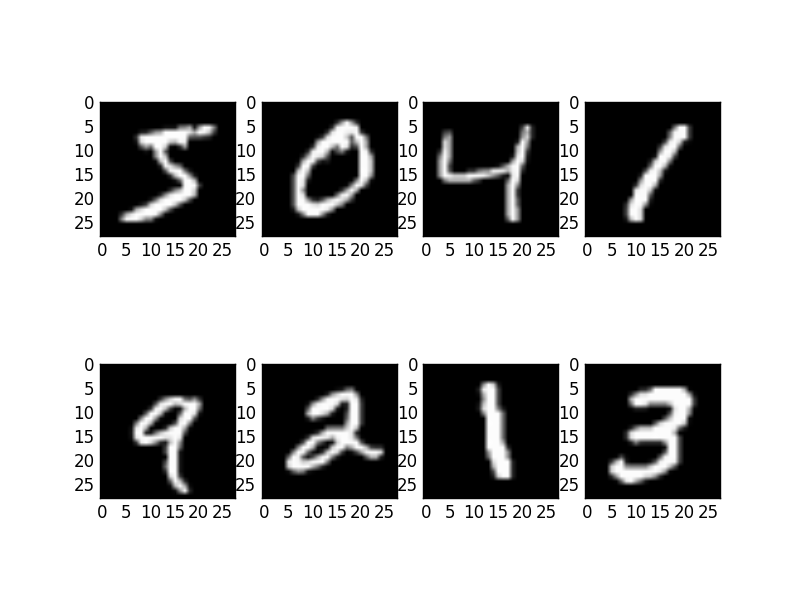
\includegraphics[width=12cm, keepaspectratio]{figures/mnist.png}
	\caption{Samples extracted from the MNIST database.}
	\label{fig:mnist}
\end{figure}

\subsection{Gradient images}\label{subsec:edge}
The first issue with \gls{mnist} database that must be addressed is that the grayscale images that it contains share similar intensity levels: a white digit over a black background. In real world, the digits can be found written in several colors over different backgrounds and the datasets must resemble every possible combination. In order to achieve that generalization, the \textbf{gradient of the images} has been calculated. The resultant samples are less dependent from the light and color conditions than the original ones, forcing the neural network to focus in the shape of the digits to classify them.

According to the study carried out by Nuria Oyaga \footnote{\url{http://jderobot.org/Noyaga-tfg\#Testing\_Neural\_Network}}, the operator that leads to better results is the \textbf{Sobel filter}. This operator approximates the gradient of an image function~\cite{sonka1999image}, convolving the image with the following kernels to highlight horizontal and vertical edges, respectively:  
\begin{equation}\label{eq:sobel}
h_x = 
\begin{bmatrix}
1 & 2 & 1\\
0 & 0 & 0\\
-1 & -2 & -1
\end{bmatrix}
,\quad
h_y = 
\begin{bmatrix}
-1 & 0 & 1\\
-2 & 0 & 2\\
-1 & 0 & 1
\end{bmatrix}
\end{equation}
The absolute values of the resultant images, $x$ and $y$, are then added, obtaining the gradient image.

\subsection{Data augmentation}
The second problem that has been detected with \gls{mnist} is that the images are \textbf{noiseless} and the digits are always centered with a scale and a rotation angle that are almost \textbf{invariant}. However, the digit classifier has to deal with noisy images that can be randomly scaled, translated and/or rotated. In order to get a database with images that look like the ones that our application is going to work with, the \gls{mnist} database must be \textbf{augmented}.

Two alternatives have been considered to solve this problem: real-time data augmentation provided by Keras and generating our own database.

\subsubsection{Real-time data augmentation with Keras}
Thanks to the \textit{.ImageDataGenerator()} method provided by Keras (see Section~\ref{subsec:utils}), the \gls{mnist} dataset can be augmented in \textbf{real-time} during training. In order to cover most of the real cases, random rotation, translation and zooming has been applied to generate new samples. In addition to that, a Sobel filtering was also applied through a user-defined function. The samples generated by the following code \footnote{\url{https://git.io/vH0qz}} can be seen in Figure~\ref{fig:aug_keras}.

\begin{lstlisting}
datagen = imkeras.ImageDataGenerator(
	                  zoom_range=0.2, rotation_range=20, width_shift_range=0.2, 
	                  height_shift_range=0.2, fill_mode='constant', cval=0,
	                  preprocessing_function=self.sobelEdges)
...	              
generator = datagen.flow(x, y, batch\_size=batch\_size)
\end{lstlisting}

\begin{figure}
	\centering
	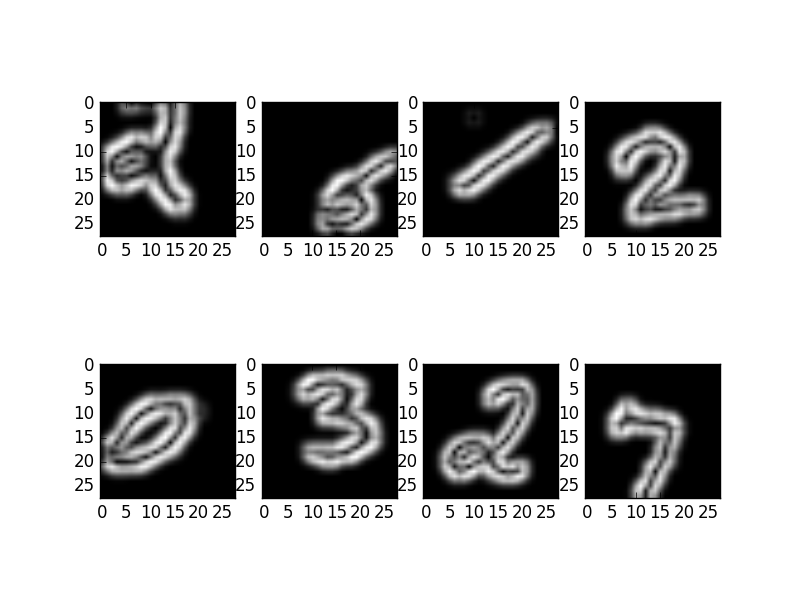
\includegraphics[width=12cm, keepaspectratio]{figures/aug_keras.png}
	\caption{Samples generated with Keras from MNIST database.}
	\label{fig:aug_keras}
\end{figure}

Besides these transformations, it's also necessary to simulate the \textbf{noise} that may be present in real images. Keras generator doesn't support the addition of noise. For this purpose, Keras includes noise layers such as the \textbf{GaussianNoise layer}, which adds Gaussian noise with a standard deviation distribution defined by the user. It's important to note that Keras treat noise layers as regularization methods that are only active during training time to avoid overfitting. In order to add noise to the generated samples, a GaussianNoise layer was established as the \textbf{input layer} of the model.

\subsubsection{Handmade augmented datasets}\label{subsec:handmade}
The alternative to real-time data augmentation with Keras is building \textbf{our own datasets} applying the previously mentioned transformations to the images. My mate Nuria Oyaga has build~5~new databases with two sets each one: training and validation \footnote{\url{http://jderobot.org/Noyaga-tfg\#Comparing_Neural_Network}}. These are the new databases: 
\begin{itemize}
	\item \textbf{Sobel}: \gls{mnist} database after applying the Sobel filter to every image.~48000~samples for traning and~12000~samples for validation. 
	\item \textbf{0-1}: Same size than Sobel database. One transformed image per every Sobel database image. Sobel database images are replaced by the the transformed ones.~48000~samples for traning and~12000~samples for validation. 
	\item \textbf{1-1}: Double size than Sobel database. One transformed image per every Sobel database image. Both Sobel database images and the transformed images are included in the~1-1~database.~96000~samples for training and~24000~samples for validation. 
	\item \textbf{0-6}: Six times the size of Sobel database. Six transformed images per every Sobel database image. Sobel database images are replaced by the transformed ones.~288000~samples for training and~72000~samples for validation. 
	\item \textbf{1-6}: Seven times the size of Sobel database. Six transformed images per every Sobel database image. Both Sobel database images and the transformed images are included in the~1-6~database.~336000~samples for training and~84000~samples for validation. 
\end{itemize}

Besides that, the test dataset of the \gls{mnist} database (10000~samples) has been converted into a~\textbf{1-6~test dataset} (70000~samples).

In Figure~\ref{fig:aug_nuria}, the first samples of every handmade dataset can be seen.

\begin{figure}
	\centering
	\begin{subfigure}{0.5\textwidth}
		\centering
		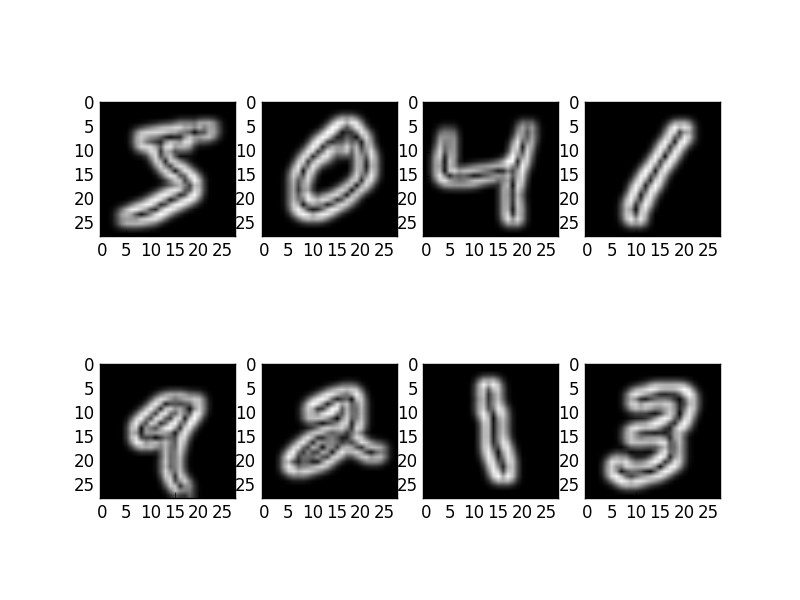
\includegraphics[width=1\linewidth]{figures/Sobel.png}
		\caption{}\label{fig:sobel}
	\end{subfigure}%
	\begin{subfigure}{0.5\textwidth}
		\centering
		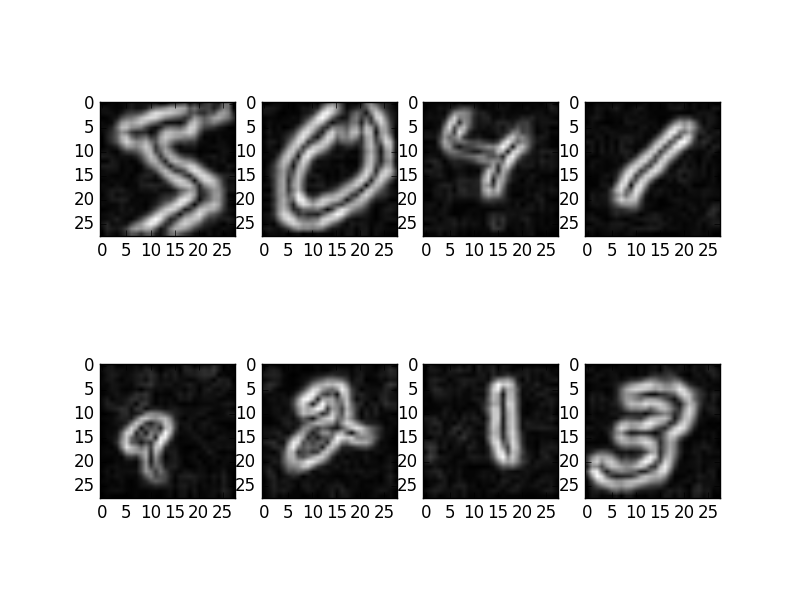
\includegraphics[width=1\linewidth]{figures/0-1.png}
		\caption{}\label{fig:0-1}
	\end{subfigure}
	\begin{subfigure}{0.5\textwidth}
		\centering
		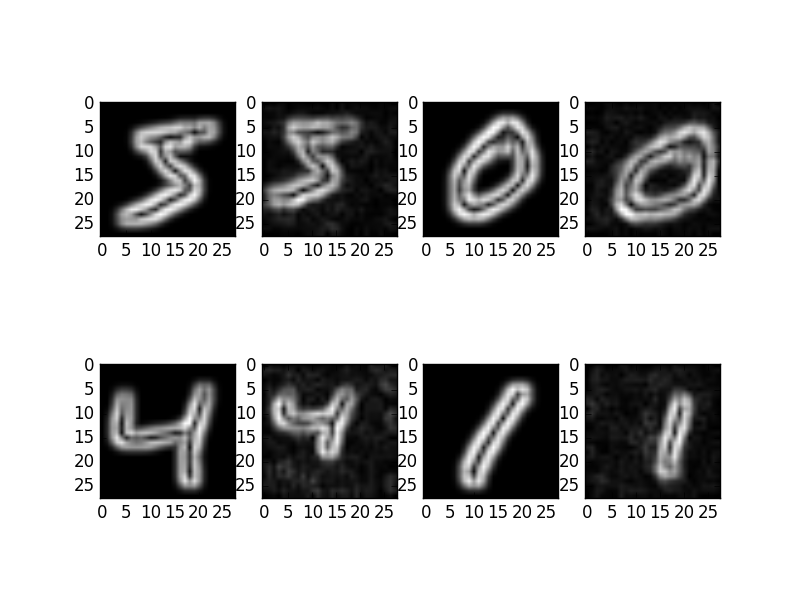
\includegraphics[width=1\linewidth]{figures/1-1.png}
		\caption{}\label{fig:1-1}
	\end{subfigure}%
	\begin{subfigure}{0.5\textwidth}
		\centering
		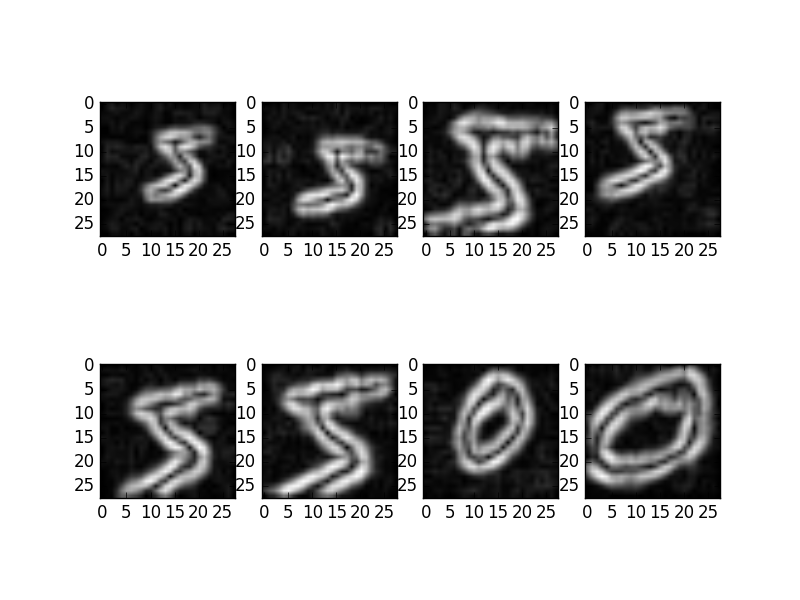
\includegraphics[width=1\linewidth]{figures/0-6.png}
		\caption{}\label{fig:0-6}
	\end{subfigure}
	\begin{subfigure}{0.5\textwidth}
		\centering
		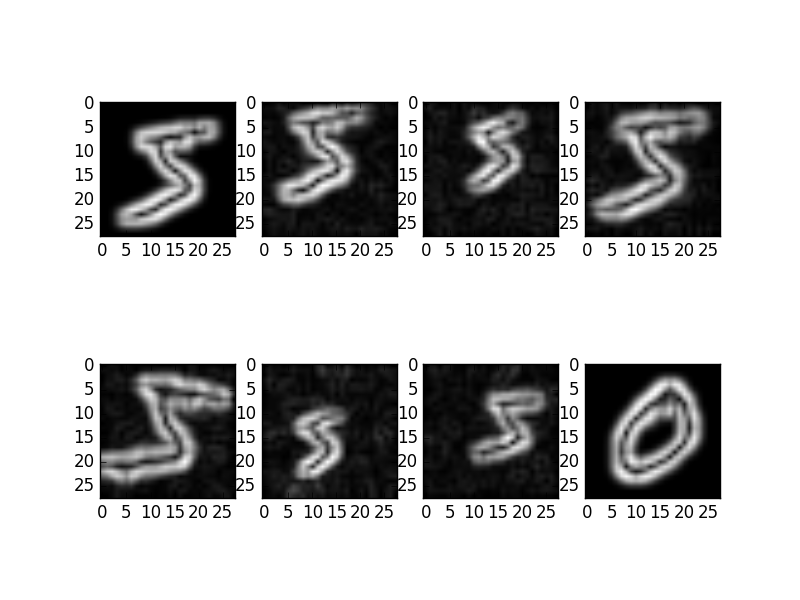
\includegraphics[width=1\linewidth]{figures/1-6.png}
		\caption{}\label{fig:1-6}
	\end{subfigure}
	\caption{First samples of handmade datasets: a) Sobel, b)~0-1, c)~1-1, d)~0-6~and e)~1-6. }
	\label{fig:aug_nuria}
\end{figure}

\subsubsection{From LMDB to HDF5} \label{subsubsec:lmdb2hdf5}
These databases were initially built to feed a \textbf{Caffe}~\cite{jia2014caffe} neural network. That's why they were saved as \textbf{\gls{lmdb} files} \footnote{\url{http://www.lmdb.tech/doc/}}. In order to make it easier to feed the Keras model, the \gls{lmdb} databases have been converted into \textbf{\gls{hdf5} files} (see Section~\ref{sec:hdf}). For this conversion, the script \textbf{\textit{datasetconversion.py}} \footnote{\url{https://git.io/vHWTe}} has been written.

\begin{itemize}
	\item \textbf{Reading the \gls{lmdb} database}. On one hand, the \gls{lmdb} library for Python \footnote{\url{https://lmdb.readthedocs.io/en/release/\#}} has been employed to open the database, initialize a cursor and iterate over each key-value pair in the database. On the other hand, \textbf{Google's Protocol Buffers}~\footnote{\url{https://developers.google.com/protocol-buffers/}} have been used to parse the data that was extracted from the database. "With protocol buffers, you write a \textit{.proto} description of the data structure you wish to store. From that, the protocol buffer compiler creates a class that implements automatic encoding and parsing of the protocol buffer data with an efficient binary format"~\cite{protobuf}. Here can be seen the \textit{.proto} file that defines the data structure used by Caffe to store the \gls{mnist} database, as obtained from~\cite{lmdb_tutorial}: 
	
\begin{lstlisting}
package datum;
message Datum {
	optional int32 channels = 1;
	optional int32 height = 2;
	optional int32 width = 3;
	// the actual image data, in bytes
	optional bytes data = 4;
	optional int32 label = 5;
	// Optionally, the datum could also hold float data.
	repeated float float_data = 6;
	// If true data contains an encoded image that need to be decoded
	optional bool encoded = 7 [default = false];
}
\end{lstlisting}
	
	Thanks to the \textit{.proto} file, the compiler generates a Python module that contains the \textbf{Datum class}. Datum class provides the \textbf{\textit{.ParseFromString()} method}, which is employed to parse the image data. Here is the resulting code:

\begin{lstlisting}
# We initialize the cursor that we're going to use to access every
# element in the dataset.
lmdb_env = lmdb.open(sys.argv[1])
lmdb_txn = lmdb_env.begin()
lmdb_cursor = lmdb_txn.cursor()

x = []
y = []
nb_samples = 0

# Datum class deals with Google's protobuf data.
datum = datum.Datum()

if __name__ == '__main__':
	# We extract the samples and its class one by one.
	for key, value in lmdb_cursor:
		datum.ParseFromString(value)
		label = np.array(datum.label)
		data = np.array(bytearray(datum.data))
		im = data.reshape(datum.width, datum.height,
		datum.channels).astype("uint8")
	
		x.append(im)
		y.append(label)
		nb_samples += 1
		
		print("Extracted samples: " + str(nb_samples) + "\n")
	
	x = np.asarray(x)
	y = np.asarray(y)
\end{lstlisting}
	
	\item \textbf{Writing the \gls{hdf5} files}. Thanks to the \textbf{h5py library~\footnote{\url{http://www.h5py.org/}}} for Python, the data extracted from the \gls{lmdb} database has been stored into a \gls{hdf5} file with two datasets: label and data. The code can be seen in the following frame:	 
	\begin{lstlisting}
	f = h5py.File("../../Datasets/" + sys.argv[2] + ".h5", "w")
	
	# We store images.
	x_dset = f.create_dataset("data", (nb_samples, datum.width,
	datum.height, datum.channels), dtype="f")
	x_dset[:] = x
	
	# We store labels.
	y_dset = f.create_dataset("labels", (nb_samples,), dtype="i")
	y_dset[:] = y
	f.close()
	\end{lstlisting}
\end{itemize} 

\subsubsection{Conclusions}
After coding and testing both implementations for augmenting the database, it has been decided to go for the \textbf{handmade datasets}. While real-time data augmentation is really useful to avoid storing all the data that is needed for training, it makes it harder to take a look into what is being fed to the network and reproduce results. Also, in this particular case, we are interested in \textbf{compare the performance} of neural networks built with different libraries, so they must be trained with the same datasets.

\section{Measuring performance}\label{sec:measuring}
The performance of the models will be evaluated using the \textit{CustomEvaluation} class and the measurements calculated with this class will be visualized using an Octave function. In this section, both of them will be described.

\subsection{\textit{CustomEvaluation} class}
\textbf{\textit{CustomEvaluation} class}~\footnote{\url{https://git.io/vQeDk}} is totally independent from Keras. It calls functions that measure the performance of the model during test and/or training time and saves them into a file which is compatible with Octave.
\begin{itemize}
	\item \textbf{Obtaining the measurements}. The user provides the real labels and the probability distribution of the predicted ones. Log loss, accuracy, precision, recall and a confusion matrix are computed. These functions are defined in Section~\ref{sec:skoctave} and Section~\ref{subsec:models}.
	\item \textbf{Storing results}. \textit{CustomEvaluation} class stores the results in a \textbf{Python dictionary}. Additionally, it can store the \textbf{learning curves} if \textit{training} option is set. In the following section, the Keras callback employed to build the learning curves will be discussed.
	\item \textbf{Python-Octave \textit{translation}}. For this task, the \textbf{SciPy library} \footnote{\url{https://docs.scipy.org/doc/scipy-0.18.1/reference/index.html}} has been used. It provides the \textit{.savemat()} method that saves Python dictionaries into Matlab \textit{.mat} files, which are also compatible with Octave (see Section~\ref{sec:skoctave}).
\end{itemize}

Here's a usage example:
\begin{lstlisting}
if training == "n":
	measures = CustomEvaluation(y_test, y_proba, training)
else:
	train_loss = learning_curves.loss
	train_acc = learning_curves.accuracy
	val_loss = validation.history["val_loss"]
	val_acc = validation.history["val_acc"]
	results = CustomEvaluation(y_test, y_proba, training, train_loss,
	train_acc, val_loss, val_acc)

results_dict = results.dictionary()
results.log(results_dict)
\end{lstlisting}

\subsubsection{\textit{LearningCurves} callback} \label{subsubsec:learningcurves}
During training time, Keras automatically saves into a \textit{.History()} object (see Section~\ref{subsec:callbacks}) the validation results obtained after every epoch. It's interesting to face these validation results with the ones obtained after every batch during training.

\textbf{\textit{LearningCurves}} \footnote{\url{https://git.io/vQeDW}} is a custom Keras callback that has been coded to save the accuracy and loss obtained after each batch into Python lists. The code below shows how it works.
\begin{lstlisting}
class LearningCurves(keras.callbacks.Callback):
''' LearningCurve class is a callback for Keras that saves accuracy
and loss after each batch.
'''    

def on_train_begin(self, logs={}):
	self.loss = []
	self.accuracy = []

def on_batch_end(self, batch, logs={}):
	self.loss.append(float(logs.get('loss')))
	self.accuracy.append(float(logs.get('acc')))
\end{lstlisting}

\subsection{Octave function}
Now that all the data has been collected, it has to be properly displayed. The function \textbf{\textit{benchmark.m}} \footnote{\url{https://git.io/vHPBt}} has been written to address this issue. It takes as its only argument the path to the \textit{.mat} file that has been generated with the \textit{CustomEvaluation} class and plots the results as they can be seen in Figure~\ref{fig:benchmark}. Additionally, it prints them to the standard output.

\begin{figure}
	\centering
	\begin{subfigure}{1\textwidth}
		\centering
		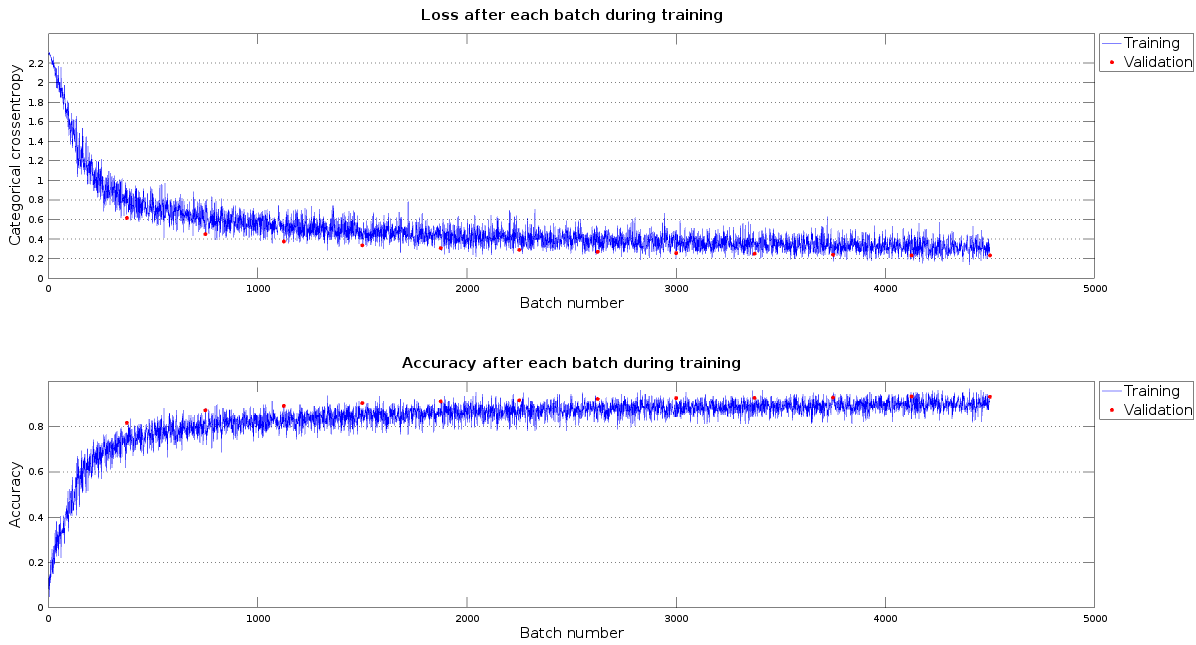
\includegraphics[width=1\linewidth]{figures/learning_curves.png}
		\caption{}
	\end{subfigure}
	\begin{subfigure}{0.5\textwidth}
		\centering
		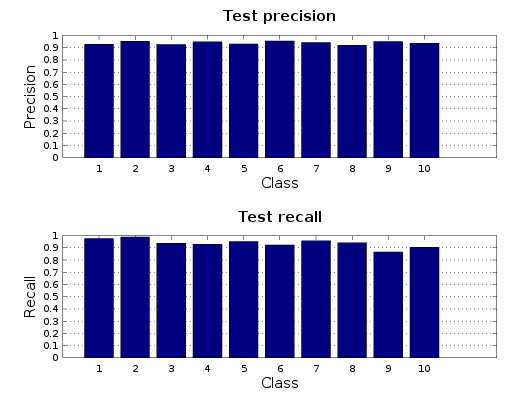
\includegraphics[width=0.9\linewidth]{figures/prec_rec.png}
		\caption{}
	\end{subfigure}%
	\begin{subfigure}{0.5\textwidth}
		\centering
		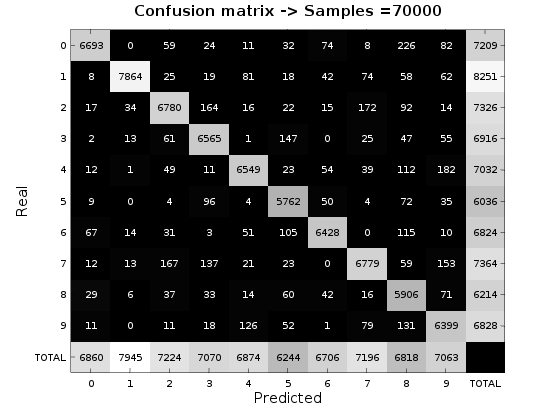
\includegraphics[width=0.9\linewidth]{figures/conf_mat.png}
		\caption{}
	\end{subfigure}
	\caption{Parameters displayed by \textit{benchmark.m}: a) learning curves, b) precision and recall and b) confusion matrix.}
	\label{fig:benchmark}
\end{figure}

\section{Convolutional layers visualization}\label{sec:visualization}
\glspl{cnn} are well-known by their ability of learning \textbf{image features}. The weights of a convolutional layer are arranged like \textbf{a set of filters}, each of which learns to identify a certain visual feature~\cite{cs231n}. As the filter is convolved with the input image, it generates an \textbf{activation map} that will tell us how that particular filter reacts to that image. In other words, the activation map will tell us whether a certain feature is present in the image or not.

In order to understand how the Keras model is learning to classify the digits, the \textbf{\textit{layer\_visualization.py}}~\footnote{\url{https://git.io/vH94o}} script has been written. This script allows the user to display the filters that are learned in every convolutional layer of the model and their resulting activation maps.

\subsection{Filters}
Keras provides a list containing every \textbf{layer object} in the model through the attribute \textit{model.layers}. Layer objects properties can be accessed thanks to the \textit{layer.get\_config()} method. Since convolutional layers in Keras are named with the prefix \textit{conv2d}, it is possible to iterate over the names of the layers looking for that prefix to find the convolutional ones, as it is shown in the code below.

\begin{lstlisting}
for i, layer in enumerate(self.model.layers):
	if layer.get_config()["name"][:6] == "conv2d":
...
\end{lstlisting}

Once the convolutional layers have been found, their \textbf{filters} are accessed through the \textit{layer.get\_weigths()} method. The matrices of weights returned by this method are reshaped to improve readability. The code that performs this operations can be seen in the following frame:

\begin{lstlisting}
shape = layer.get_weights()[0].shape
weights = layer.get_weights()[0].reshape(shape[2], shape[0],
                                              shape[1], shape[3])
\end{lstlisting}

Finally, the filters are plotted thanks to the \textbf{Matplotlib library}~\footnote{\url{https://matplotlib.org/}} for Python. The shape and the maximum/minimum values of the weights are printed to the standard output. An example of how the filters are plotted can be seen in the following chapter in Figure~\ref{fig:filters}

\subsection{Activation maps}
The output of each convolutional layer is formed by as many \textbf{activation maps} as filters have the layer. In order to get the values of these activation maps, \textbf{truncated versions} of the original model are generated, as it is shown in Figure~\ref{fig:truncated}. When a prediction is made with these truncated models, they output the activation maps that correspond to their last layer. The code which obtains the activation maps can be seen in the follwing frame:
\begin{lstlisting}
truncated = Model(inputs=self.model.inputs,
                    outputs=layer.output)
activations = truncated.predict(self.im)
\end{lstlisting}

\begin{figure}
	\begin{subfigure}{0.5\textwidth}
		\centering
		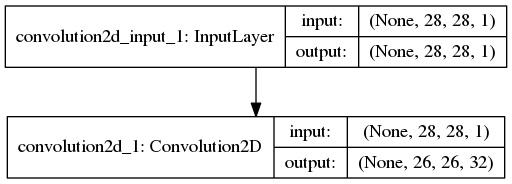
\includegraphics[width=0.9\linewidth]{figures/1stconvarch.png}
		\caption{}
	\end{subfigure}
	\begin{subfigure}{0.5\textwidth}
		\centering
		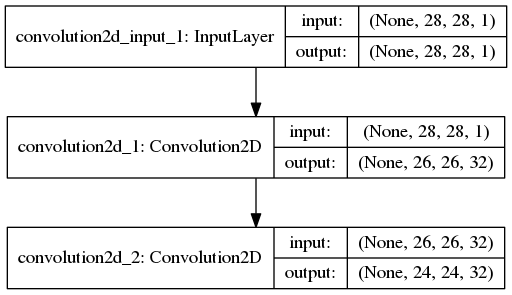
\includegraphics[width=0.9\linewidth]{figures/2ndconvarch.png}
		\caption{}
	\end{subfigure}
	\caption{Truncated versions of the model: a) one convolutional layer and b) two convolutional layers}
	\label{fig:truncated}
\end{figure}

The activation maps are plotted using the Matplotlib library as well, and their shape and maximum/minimum values are also printed to the standard output. An example of how the activation maps are plotted can be seen in the following chapter in Figure~\ref{fig:activation_maps}.

\lhead[]{CHAPTER \thechapter. EVALUATION}
\chapter{Evaluation}\label{sec:new_models}
The \gls{cnn} analyzed in Section~\ref{sec:understanding} is going to be taken as a starting point to build \emph{new models}. These models will be trained with different datasets and regularization methods and, finally, new architectures will be implemented. In this chapter, the tools developed in Chapter~\ref{ch:benchmark} will be employed to evaluate the results achieved by each \gls{cnn}. These tests will serve as a way to study the effects of the learning process in these algorithms. Before talking about the \emph{performance} of the new models, the visualization of the convolutional layers filters and activation maps is going to be analyzed.

\section{Convolutional layers visualization}
The filters and activation maps discussed in this section belong to the convolutional layers of the \emph{\textit{0-1; Patience=2} model} that can be found in Section~\ref{subsec:early_stopping}. This model has been trained with the \textit{0-1} dataset (see Section~\ref{subsec:handmade}) and an early stopping rule with patience~2. Its architecture corresponds to the one defined in Section~\ref{sec:understanding}. In order to generate the activation maps, the model will be fed with a sample extracted from the \textit{0-1} dataset. It can be seen in Figure~\ref{fig:sample}.
\begin{figure}
	\centering
	\includegraphics[width=0.3\linewidth, keepaspectratio]{figures/0-1_sample.png}
	\caption{Sample employed to generate the activation maps.}
	\label{fig:sample}
\end{figure}

\subsection{Filters}
When loading the weights of the \emph{first convolutional layer}, a Numpy array of shape~(1,~3,~3,~32) is obtained. This means that the weights are arranged in~32~filters of size~3x3. In this case, the input is a grayscale image, so the filters only have one channel (i.e. depth=1). Besides that, when examining their values, \emph{negative and positive coefficients} are found.

In Figure~\ref{fig:filters}, these filters are plotted. Some of the filters look too noisy to tell which kind of feature they are looking for. However, a few of them can be interpreted at first sight as follows:
\begin{itemize}
	\item \textbf{Horizontal edge-emphasizing filter}: filters~7,~9~and~23.
	\item \textbf{Vertical edge-emphasizing filter}: filters~8,~15~and~31.	
\end{itemize}

\begin{figure}
	\centering
	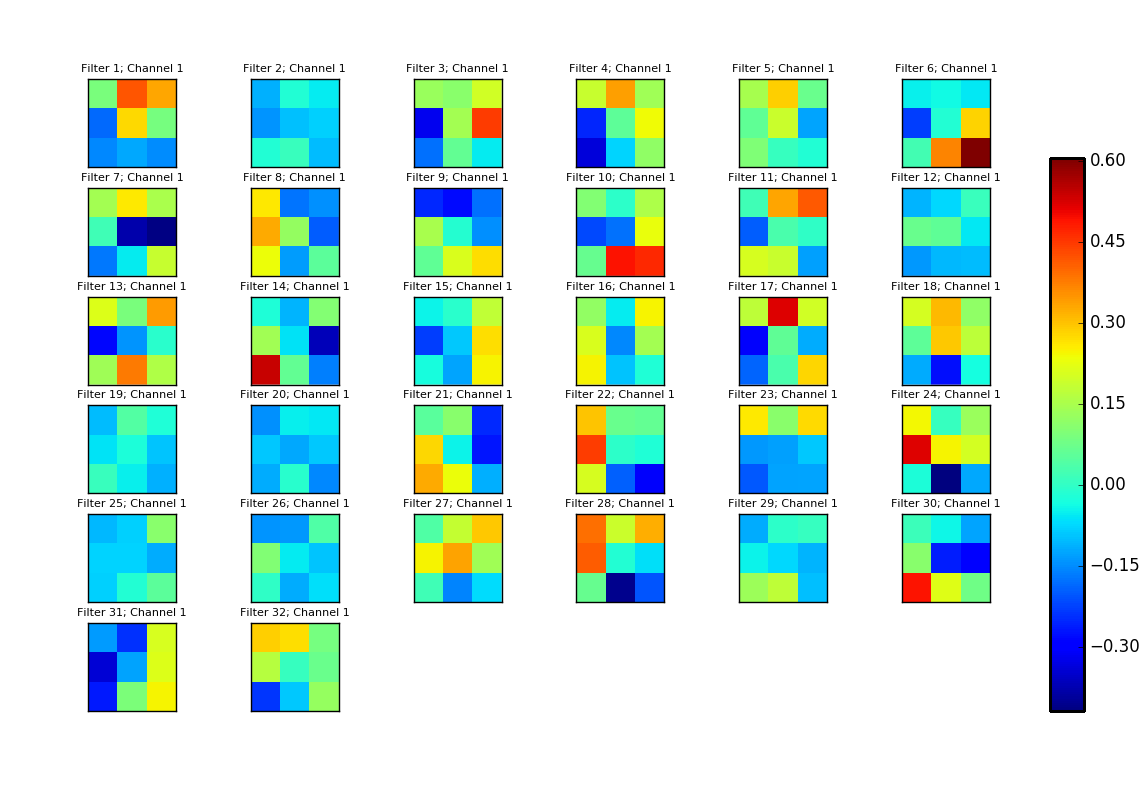
\includegraphics[width=0.92\linewidth, keepaspectratio]{figures/weights_conv2d_1.png}
	\caption{Filters of the first convolutional layer.}
	\label{fig:filters}
\end{figure}

The filters in the \emph{second convolutional layer} have been displayed as well. The weights in this layer are stored in a Numpy array of shape~(32,~3,~3,~32), which means that there are~32~filters with size~3x3~as well. However, this time their depth is~32, since there is one channel per activation map generated by the previous layer. As we get deeper in the \gls{cnn} and the dimensionality grows, the filters look noisier and become harder to interpret, as it is shown in Figure~\ref{fig:filters2}.
\begin{figure}
	\centering
	\includegraphics[width=1\linewidth, keepaspectratio]{figures/weights_conv2d_2_mod.png}
	\caption{Filters of the second convolutional layer.}
	\label{fig:filters2}
\end{figure}

\subsection{Activation maps}
Figure~\ref{fig:activation_maps} shows the activation maps that the \emph{first convolutional layer} of the model outputs. There are \emph{horizontal and vertical edge images} that confirm the interpretation of the filters given in the previous section. Besides that, some activation maps (2,~12,~19,~25~and~26) look \textit{dead}. If we look back into Figure~\ref{fig:filters}, these activation maps correspond to filters with \emph{almost flat coefficients}. This may be a signal of a high learning rate~\cite{cs231n}. In this case, the learning rate is not explicitly declared, because the ADADELTA optimizer uses an adaptive one.
\begin{figure}
	\centering
	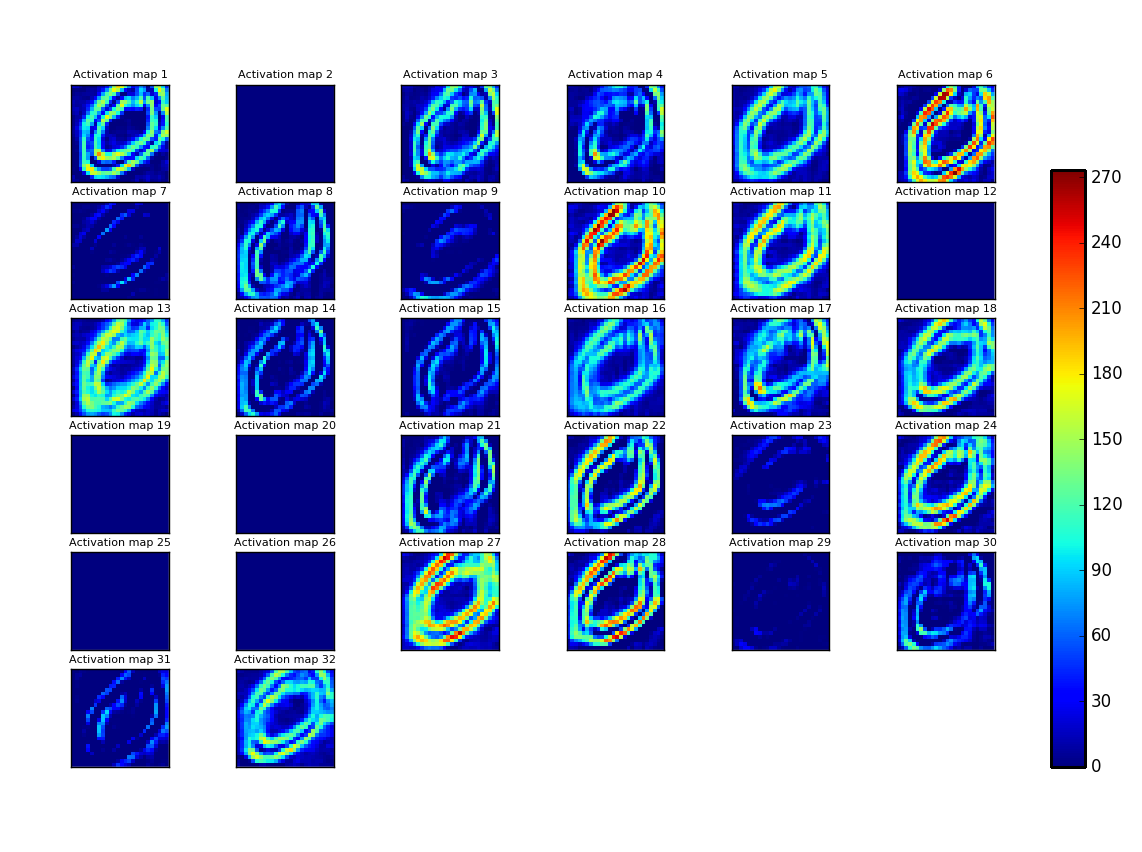
\includegraphics[width=0.9\linewidth, keepaspectratio]{figures/activation_maps_conv2d_1.png}
	\caption{Activation maps of the first convolutional layer.}
	\label{fig:activation_maps}
\end{figure}

The activation maps of the \emph{second layer} are shown in Figure~\ref{fig:activation_maps2}. The images obtained look \emph{more specialized} than the ones in the previous layer. It's easier to tell to what kind of feature (e.g. edges and corners) each activation map is responding to.
\begin{figure}
	\centering
	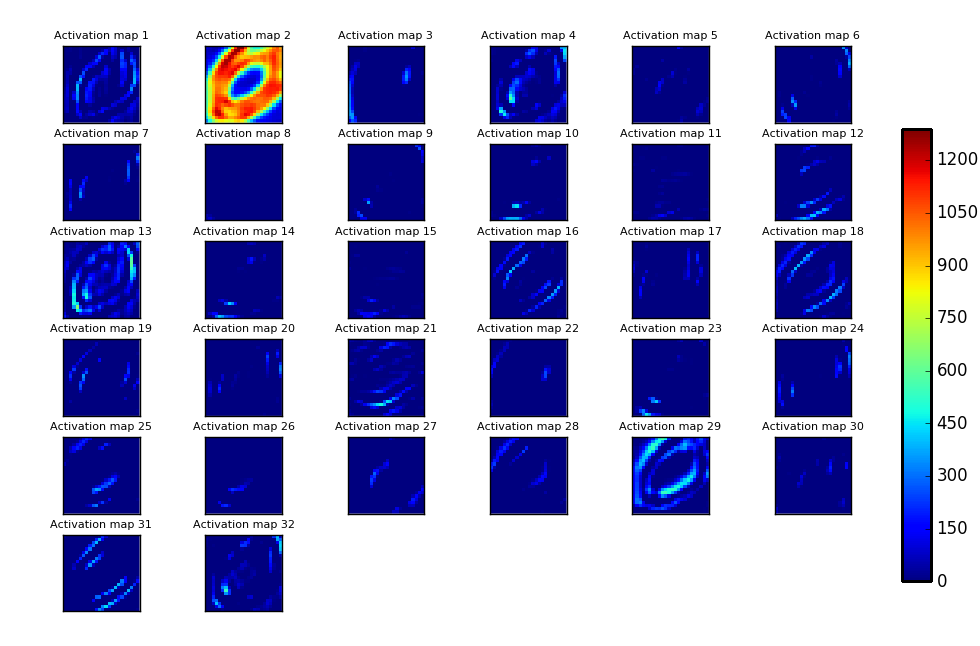
\includegraphics[width=0.9\linewidth, keepaspectratio]{figures/activation_maps_conv2d_2.png}
	\caption{Activation maps of the second convolutional layer.}
	\label{fig:activation_maps2}
\end{figure}

It's important to note that the values of the activation maps are \emph{always positive}, even if the filters have negative coefficients. This is because the \gls{relu} activation function (see Equation~\ref{eq:relu}) turn all the negative values to zero.

\section{Augmented datasets}\label{sec:new_datasets}
The original model has been trained with each of the \emph{handmade datasets} described in Section~\ref{sec:datasets}. The number of epochs has been set to~12~and the evaluation has been carried out with the~\emph{1-6~test dataset}. The results that can be seen in Table~\ref{tbl:datasets} lead to the following conclusions:
\begin{itemize}
	\item As it might be expected, the results when training with the \emph{Sobel dataset} are much worse than the ones obtained with the other datasets, because we're testing with noisy images a \gls{cnn} trained with noiseless samples.
	\item The \emph{\textit{0-6} and \textit{1-6} models} are the ones that achieve better results, as they have been trained with much more samples than \textit{0-1} and \textit{1-1}.
	\item When \emph{comparing \textit{0-1} with \textit{1-1} and \textit{0-6} with \textit{1-6}}, it can be seen that the performance is almost the same, which means that the gradient image without noise and transformations is not adding much information to the model.
\end{itemize}
In Figure~\ref{fig:val_datasets}, the validation results obtained after every epoch when training the model with each dataset can be seen.
\begin{figure}
	\centering
	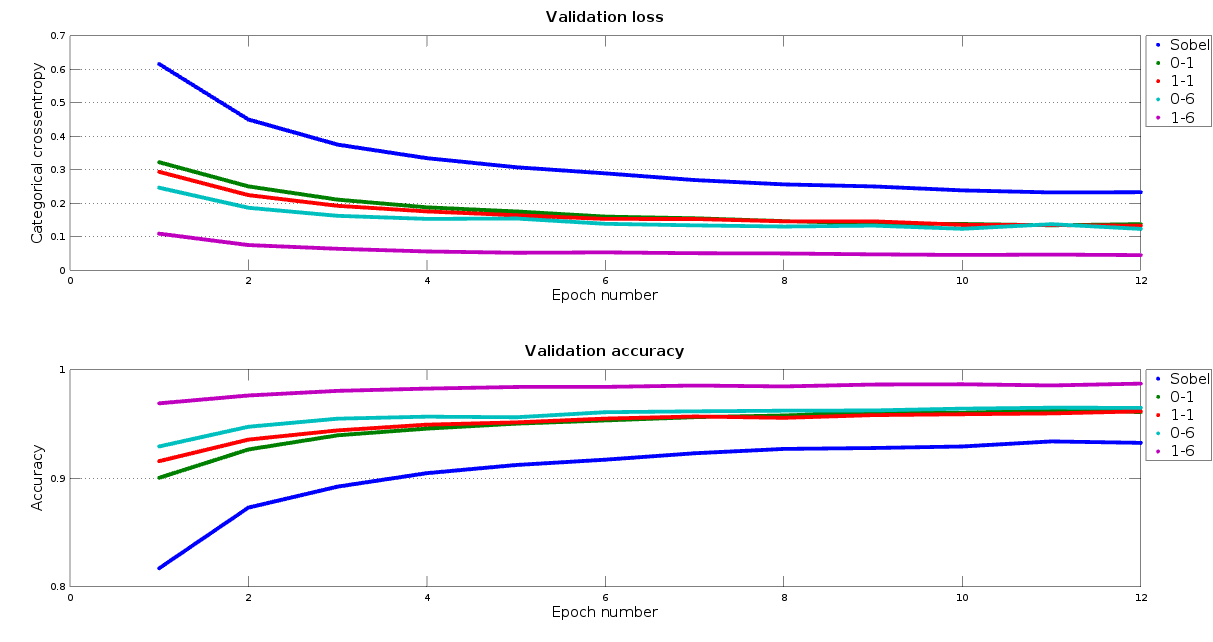
\includegraphics[width=1\linewidth, keepaspectratio]{figures/val_datasets.png}
	\caption{Validation results when training the model with different datasets.}
	\label{fig:val_datasets}
\end{figure}

Taking all of this into account, it has been decided to keep working with the \emph{\textit{0-1} model}, which achieves a performance that is comparable with the other models with the advantage of a much lower computational cost.

\begin{table}
	\centering
	\begin{tabular}{l*{4}{c}r}
		\textbf{Model} & \textbf{Loss} & \textbf{Accuracy} & \textbf{Epochs} \\
		\hline
		Sobel & 1.233 & 0.699 & 12 \\
		0-1 & 0.201 & 0.939 & 12 \\
		1-1 & 0.189 & 0.943 & 12 \\
		0-6 & 0.109 & 0.968 & 12 \\
		1-6 & 0.111 & 0.967 & 12 \\
	\end{tabular}
	\caption{Results of training with different datasets.}
	\label{tbl:datasets}
\end{table}

\section{Regularization methods}
``\emph{Regularization} is any modification we make to a learning algorithm that is intended to reduce its \emph{generalization error} but not it's training error"~\cite{Goodfellow-et-al-2016}. Reducing the generalization error is important because, even if a model achieves a great accuracy or loss with the training dataset, if it doesn't generalize well enough, the results during validation and test time won't be optimal. This is specially significant in our case, since the predictions of the digit classifier will be based on images that differ a lot from the training dataset. In this section, the effects of applying to the \emph{\textit{0-1} model} two regularization techniques (early stopping and dropout) are going to be evaluated. 

\subsection{Early stopping}\label{subsec:early_stopping}
The models in the previous section have been trained for~12~epochs. However, if we look at the \emph{validation results} in Figure~\ref{fig:val_datasets}, it can be assumed that the models were \emph{not overfitting} yet, because the results didn't stop improving. This means that they were not being trained as much as possible. Setting an \emph{early stopping} rule (see Section~\ref{subsec:callbacks}) allows training the \gls{cnn} right until it starts to overfit, making the most of it. The criteria that has been used depends on the loss during validation. The model is trained until the \emph{log loss} (see Section~\ref{eq:categorical_crossentropy}) has not improved after two validations in a row, which means a \textit{patience} of 2. Besides that, in order to keep the best \textit{version} of the model, the log loss is checked after each epoch and, if the value is lower than the previous best log loss achieved, the weights of the model are saved, overwritting the weights of the previous best \textit{version}. The difference between training the model with and without early stopping can be seen in Table~\ref{tbl:earlystopping}.
\begin{table}
	\centering
	\begin{tabular}{l*{4}{c}r}
		\textbf{Model} & \textbf{Loss} & \textbf{Accuracy} & \textbf{Epochs} \\
		\hline
		0-1 & 0.201 & 0.939 & 12 \\
		0-1; Patience=2 & 0.155 & 0.954 & 30 \\
	\end{tabular}
	\caption{Results of training with and without early stopping.}
	\label{tbl:earlystopping}
\end{table}

Early stopping means an improvement of 1.6\% in accuracy and 4.6\% in log-loss. The model has been trained for~30~epochs and it reached its best \textit{version} at the 27$^{th}$ epoch. Setting a longer \textit{patience} has been considered, but it has been decided to apply it only to the best model obtained in Section~\ref{subsec:arch} to reduce the computational cost.

\subsection{Dropout}
The models that have already been evaluated insert \emph{dropout} (see Section~\ref{subsec:layers}) before every dense layer of the \gls{cnn} (0.25\% and 0.5\%, respectively). Dropout is usually applied just to fully-connected or \emph{dense layers}, because convolutional layers are less likely to overfit due to their architecture. In order to determine how dropout affects the performance of the \glspl{cnn}, the \emph{\textit{0-1; Patience=2} model}, defined in the previous section, has been trained with and without the mentioned dropout. The results can be seen in Table~\ref{tbl:dropout}. 
\begin{table}
	\centering
	\begin{tabular}{l*{4}{c}r}
		\textbf{Model} & \textbf{Loss} & \textbf{Accuracy} & \textbf{Epochs} \\
		\hline
		No dropout & 0.189 & 0.945 & 9 \\
		Dropout & 0.155 & 0.954 & 30 \\
	\end{tabular}
	\caption{Results of training with and without dropout.}
	\label{tbl:dropout}
\end{table}

Without dropout, the model has stopped training after~9~epochs. It has \emph{learned faster}, but it has started \emph{overfitting} earlier, resulting in worst results that the ones achieved by the model trained with dropout. This can be clearly seen in Figure~\ref{fig:comp_dropout}
\begin{figure}
	\centering
	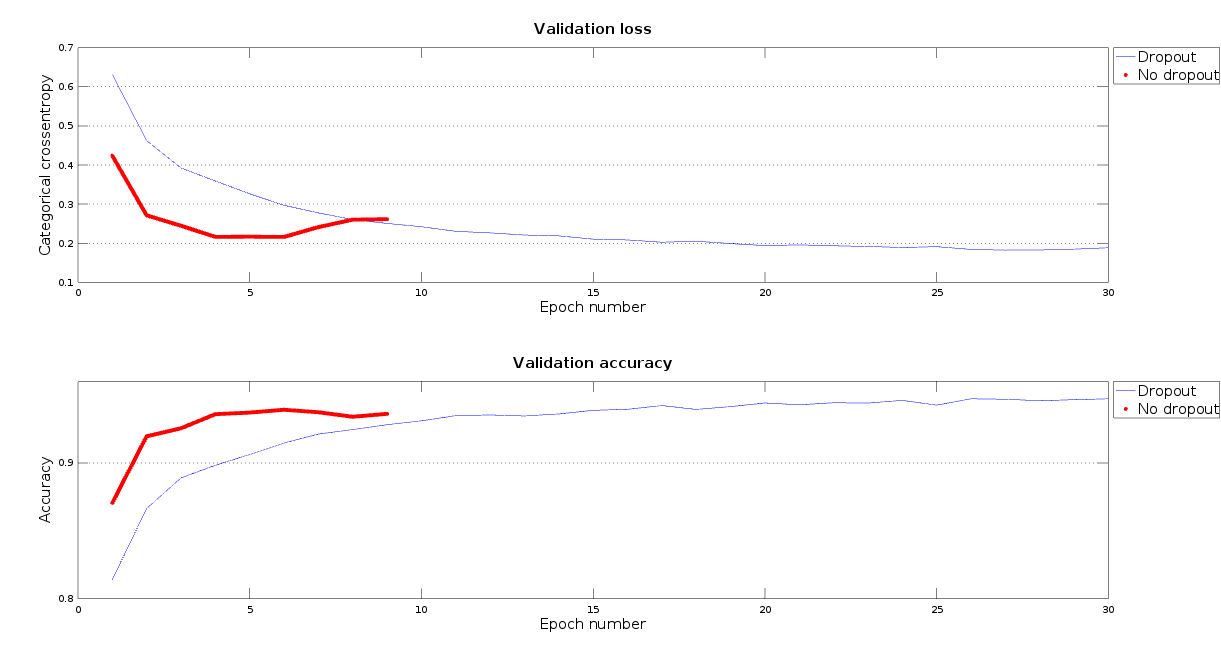
\includegraphics[width=1\linewidth, keepaspectratio]{figures/comp_dropout.png}
	\caption{Validation results with and without dropout.}
	\label{fig:comp_dropout}
\end{figure}

Additionally, in Figure~\ref{fig:lc_dropout}, the learning curves of both models can be seen. It's worth looking into these plots to realize that validation results are better than training results when the model is trained with dropout. This may seem illogical, as the \gls{cnn} should always perform better with samples that it has already seen. However, it's important to remember that dropout only applies during training and, as it will \textit{switch-off} a lot of weights in the \gls{cnn}, much of its prediction power will be lost. During validation, there are no \textit{switched-off} weights, which allows the \gls{cnn} to make better predictions. Besides that, in the figure can be seen that the training results are better when the model is trained without dropout, while the validation results are better with dropout. This means that the model with dropout is \emph{generalizing} better than the one without dropout. 
\begin{figure}
	\begin{subfigure}{1\textwidth}
		\centering
		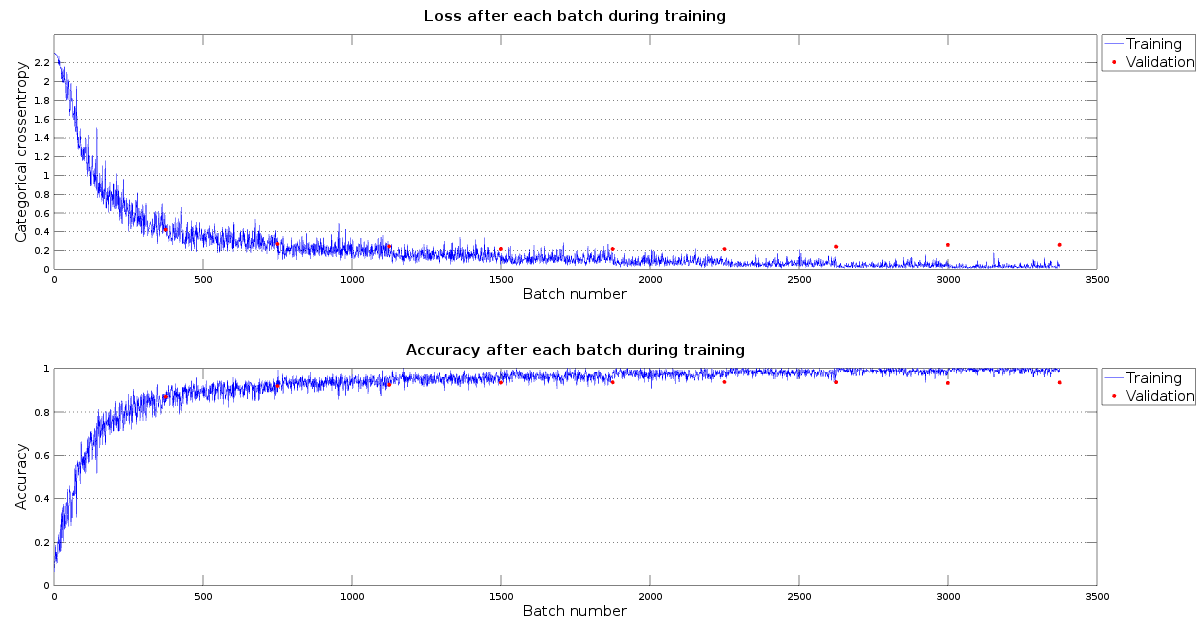
\includegraphics[width=1\linewidth]{figures/lc_nodropout.png}
		\caption{}
	\end{subfigure}
	\begin{subfigure}{1\textwidth}
		\centering
		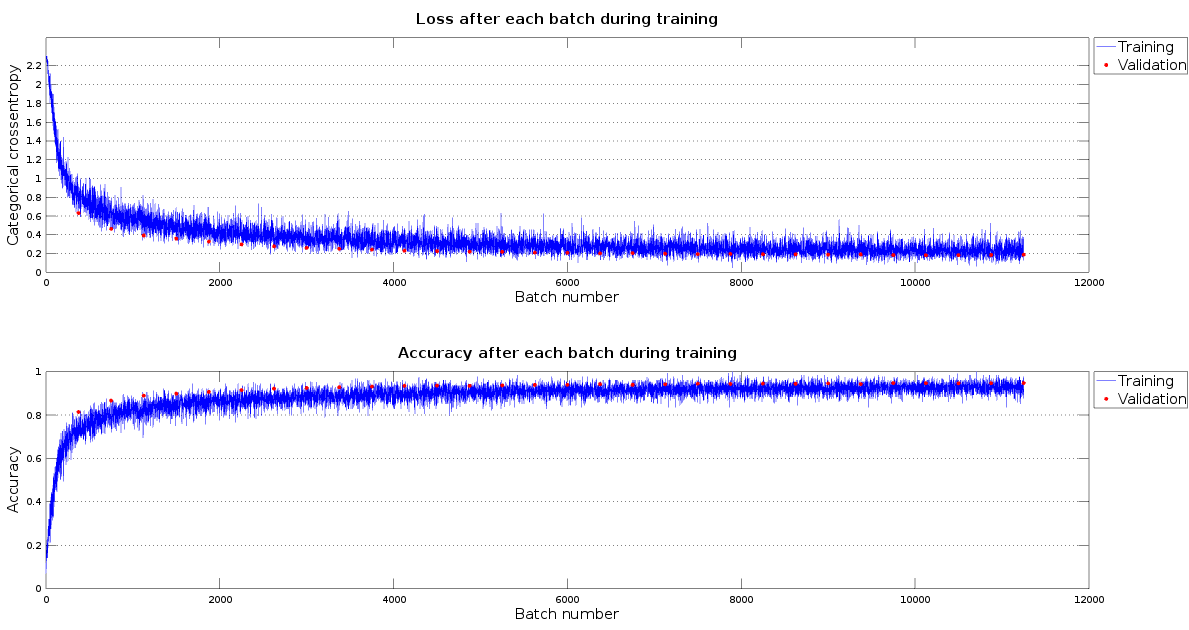
\includegraphics[width=1\linewidth]{figures/lc_dropout.png}
		\caption{}
	\end{subfigure}
	\caption{Learning curves: (a) without dropout; (b) with dropout.}
	\label{fig:lc_dropout}
\end{figure}

\section{New architectures}\label{subsec:arch}
In order to check the influence of \emph{different architectures} in the performance of the \gls{cnn}, new models with a different number of convolutional layers have been trained and tested. The stopping rule used in these trainings is the one defined in Section~\ref{subsec:early_stopping} and dropout is also applied. The decision of adding \emph{pooling layers} to the models (see Section~\ref{subsec:layers}) has been taken to reduce computational cost. In the first attempt at training a model with~6~convolutional layers, the model with~2~convolutional layers and one \emph{MaxPooling layer} was triplicated. However, the first MaxPooling layer of the model was removed because the model ended up working with an empty image:~0x0~size.
\begin{table}
	\centering
	\begin{tabular}{l*{4}{c}r}
		\textbf{Model} & \textbf{Loss} & \textbf{Accuracy} & \textbf{Epochs} \\
		\hline
		1Conv+MaxPooling & 0.191 & 0.945 & 47 \\
		2Conv+MaxPooling & 0.155 & 0.954 & 30 \\
		3Conv+MaxPooling & 0.129 & 0.945 & 28 \\
		2Conv+MaxPooling+2Conv+MaxPooling & 0.092 & 0.970 & 27 \\
		4Conv+MaxPooling+2Conv+MaxPooling & 0.092 & 0.971 & 24 \\
	\end{tabular}
	\caption{Results of training models with different architectures.}
	\label{tbl:arch}
\end{table}

As it is shown in Table~\ref{tbl:arch}, the best results have been obtained with the models that contain~4~and~6~convolutional layers. Besides that, taking a look into the validation curves (see Figure~\ref{fig:comp_arch}), it can be assumed that when the number of layers is increased, the neural network tends to lead to better results with less epochs.

\begin{figure}
	\centering
	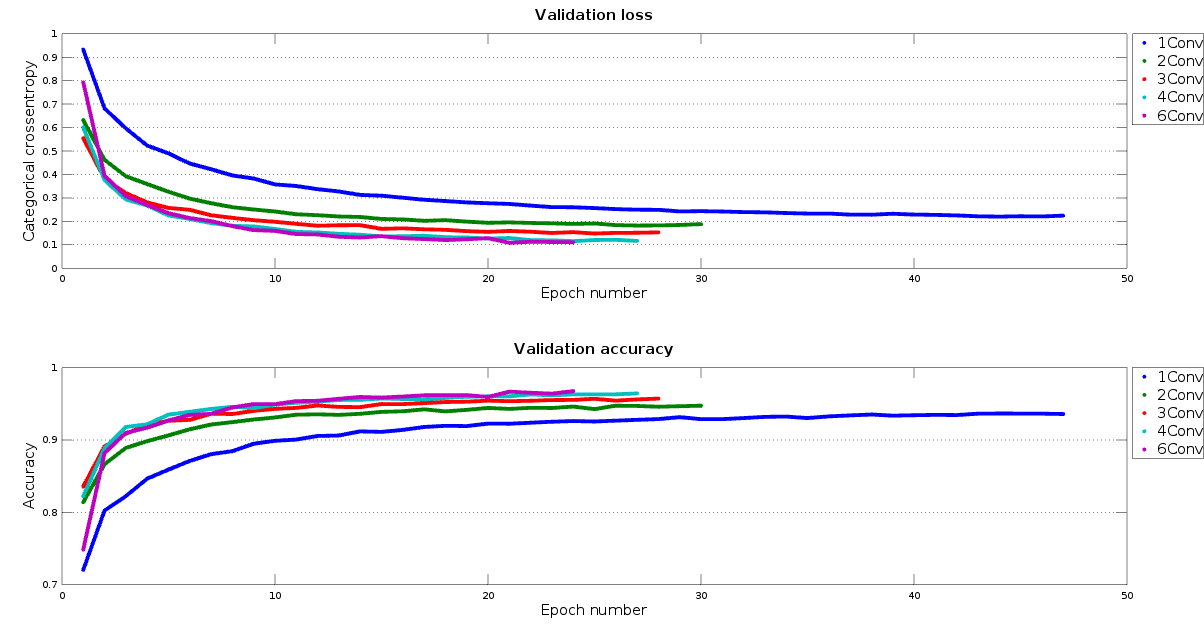
\includegraphics[width=1\linewidth, keepaspectratio]{figures/full_comparison.png}
	\caption{Validation results with different architectures.}
	\label{fig:comp_arch}
\end{figure}

The model with~6~layers has a slightly better accuracy, but a slightly worse loss, than the one with~4~layers. Considering that computational cost is higher when training the \textit{6Conv} model, the \emph{\textit{4Conv} model} seems to be the best bet. In order to make the most of it, it has been trained again but increasing the \emph{\textit{patience}} of the early stopping rule from~2~to~5. The results obtained with this new stopping rule can be seen in Table~\ref{tbl:arch_patience5}. These results imply that being more \textit{patient} during training can lead to a better performance, although in this case the improvement is not very significant.
\begin{table}
	\centering
	\begin{tabular}{l*{4}{c}r}
		\textbf{Model} & \textbf{Loss} & \textbf{Accuracy} & \textbf{Epochs} \\
		\hline
		4Conv; Patience=2 & 0.092 & 0.970 & 27 \\
		4Conv; Patience=5 & 0.082 & 0.973 & 37 \\
	\end{tabular}
	\caption{\textit{4Conv} model trained with different stopping rules.}
	\label{tbl:arch_patience5}
\end{table}

A visualization of the performance achieved by the best model built in this project (i.e. \emph{4Conv; Patience=5 model}) is shown in Figure~\ref{fig:best}. The Octave function discussed in Section~\ref{subsec:octave-func} has been employed to generate the plots displayed in this figure.

\begin{figure}
	\centering
	\begin{subfigure}{1\textwidth}
		\centering
		\includegraphics[width=1\linewidth]{figures/lc_42.png}
		\caption{}
	\end{subfigure}
	\begin{subfigure}{0.5\textwidth}
		\centering
		\includegraphics[width=0.9\linewidth]{figures/pr_42.png}
		\caption{}
	\end{subfigure}%
	\begin{subfigure}{0.5\textwidth}
		\centering
		\includegraphics[width=0.9\linewidth]{figures/cm_42.png}
		\caption{}
	\end{subfigure}
	\caption{Performance of \textit{4Conv; Patience=5} model: (a) learning curves; (b) precision and recall; (c) confusion matrix.}
	\label{fig:best}
\end{figure}
\lhead[]{CHAPTER \thechapter. CONCLUSIONS}
\chapter{Conclusions}\label{ch:conclusions}
In this chapter, we are going to recall the main conclusions reached during the development of this project. These conclusions will be divided following the \emph{sub-objectives} defined in Section~\ref{sec:objectives}. After summarizing the conclusions, suggestions for future works will be proposed.

\section{Conclusions}
\subsection*{Deep understanding of CNNs built with Keras}
\begin{itemize}
	\item The input data in Keras models are usually provided as \emph{\gls{hdf5} files}, which can be imported as Numpy arrays that can be easily accessed and reshaped. \gls{hdf5} is also employed by Keras to save the models.
	\item \glspl{cnn} are built in Keras as a stack of \emph{fully configurable modules} (convolutional layers, regularization layers, activation functions...) which can be easily modified when needed, allowing fast experimentation.
	\item The core elements of a \gls{cnn} are convolutional and pooling layers combined with non-linear activation functions (e.g. \gls{relu}), which altogether allow the learning of \emph{complex image features} in a hierarchical way with a reasonable computational cost.
	\item In \emph{classification tasks}, the output layer of the model must be, at least, one fully-connected layer with as many neural units as classes the problem has. The activation function employed in this layer (e.g. Softmax) transforms the output into a probability distribution.
	\item The cost function and optimizer of the \emph{learning process} can be easily configured. Moreover, Keras allows the addition of callbacks which can monitor the state and the performance of the \gls{cnn} at given stages of the training process.
	\item Keras provides tools for \emph{image preprocessing} that can be used to generate new data in real-time. This is useful for augmenting the database without storing the new samples.
\end{itemize}

\subsection*{Test bench tools}
\begin{itemize}
	\item The creation of a test bench for \emph{comparing results} has improved the speed of the experimentation and the interpretability of the obtained results.
	\item Employing \emph{handmade augmented datasets} instead of real-time data augmentation has allowed an easier control of what we have fed to the \glspl{cnn}.
	\item \emph{Scikit-learn library} provides a wide variety of functions for evaluating \glspl{cnn}. Besides that, it is independent from Keras, which allows the comparison of the results obtained with models built with different platforms like Caffe.
	\item Building \emph{a bridge from Python to Octave} with the SciPy library has opened the doors to the powerful visualization tools provided by Octave.
	\item The modular logic employed by Keras allows to easily look into the inner parts of the models, which has been very useful for \emph{visualizing the activation maps and filters} of the convolutional layers.
\end{itemize}

\subsection*{Effects of the learning process in \glspl{cnn} performance}
\begin{itemize}
	\item While training the \gls{cnn} with the \emph{original \gls{mnist} database} leads to impressive accuracy in test time, the model generated doesn't generalize well enough when it is evaluated with real-world images.
	\item Training with \emph{gradient images} instead of the original ones makes the \gls{cnn} more robust with respect to the light and color conditions.
	\item The \emph{datasets augmented} with random transformations enable a better generalization, which means a significant improvement with real-world images.
	\item The models trained with \emph{dropout} learn slower and have worse results during training that the ones trained without dropout, but perform much better in validation and test time. This means that the \glspl{cnn} trained with dropout generalize better. 
	\item Setting a good \emph{early stopping} rule is critical to make the most of the training process. 
	\item The analysis of the \emph{activation maps} has proved that the \gls{cnn} is learning mostly features about the edges of the samples. It's easier to see this trend in the activation maps of the last convolutional layer.
	\item Some activation maps look \textit{dead}, which could mean that the learning rate is too high according to some researchers~\cite{cs231n}.
	\item The \emph{filters} in the first layer can be related with their activation maps. However, when we go deeper into the network, the dimensionality grows too much to easily interpret the filters and they look noisier. 
\end{itemize}

\subsection*{JdeRobot component for digit classification}
\begin{itemize}
	\item The \emph{image acquisition} from different video streams has been easily solved using the \textit{cameraserver} driver provided by JdeRobot framework.
	\item On one hand, capturing images from \emph{smartphone cameras} instead of webcams has made the application much more flexible than before. On the other hand, the frame rate is significantly higher with webcams.
	\item The use of \emph{threads} for the different tasks of the component is essential for enabling real-time execution.
	\item The performance of the component has been highly improved after replacing the \gls{cnn} of the Keras example analyzed in Section~\ref{sec:understanding} with the \emph{\textit{4Conv; Patience=5} model} evaluated in Section~\ref{subsec:arch}.
\end{itemize}

\section{Future works}
The understanding of the \glspl{cnn} acquired in this project opens the door to the application of new algorithms in \emph{more complex real-world problems}. For instance, they can be used not only for object classification, but also for \emph{object detection}. Algorithms based in \glspl{cnn} have shown a great performance in classical benchmarks like Pascal VOC\footnote{\url{http://host.robots.ox.ac.uk/pascal/VOC/databases.html}} and COCO\footnote{\url{http://mscoco.org/}}. Deep learning libraries like Keras and Caffe provide pre-trained weights for popular neural networks trained with these databases, allowing the user to fine-tune the models with new samples. The main difficulty that has to be faced in object detection is the high computational cost, but some algorithms are achieving real-time or almost \emph{real-time predictions} (e.g. YOLO\footnote{\url{https://pjreddie.com/darknet/yolo/}} and SSD\footnote{\url{https://github.com/weiliu89/caffe/tree/ssd}}). Possible applications of these kind of algorithms are autonomous driving, video surveillance and face recognition. In particular, in autonomous driving we can find them coping with problems like steering angle prediction and vehicle detection (see Figure~\ref{fig:vehicle}).
\begin{figure}
	\centering
	\includegraphics[width=0.8\linewidth, keepaspectratio]{figures/cars.jpg}
	\caption{Vehicle detection with YOLO applied to Udacity's self-driving car dataset (source\cite{udacity}).}
	\label{fig:vehicle}
\end{figure}

Another interesting field of study is to estimate the pose of the human body from video images. In that sense, convolutional pose machines are achieving very promising results~\cite{DBLP:journals/corr/WeiRKS16}. These algorithms can be used to better understand body language.

Besides the possible applications in computer vision, \glspl{cnn} can also be employed to solve tasks like speech recognition~\cite{conf/icassp/Abdel-HamidMJP12} and natural language processing~\cite{DBLP:journals/corr/LopezK17}.

%%%%%%%%%%%%%%% Bibliography %%%%%%%%%%%%%%%
\printbibliography

\end{document}